\documentclass[output=paper]{langsci/langscibook}
\ChapterDOI{10.5281/zenodo.3929247}

\markuptitle{German \textit{noch} under reanalysis}{German noch under reanalysis}
\renewcommand{\lsChapterFooterSize}{\small} %footers in editedvolumes
\renewcommand{\lsCollectionPaperFooterTitle}{German \noexpand\textit{noch} under reanalysis}
\author{Martin Kopf-Giammanco\affiliation{Universität des Saarlandes}}

% \epigram{}

\abstract{This paper investigates (i) the semantics of present day German \textit{noch} in comparative readings. In doing so it (ii) presents experimental work on comparative \textit{noch}'s presuppositional meaning component. In the second part, I will (iii) provide a survey of diachronic data from the Old German period and (iv) propose a process of reanalysis for the comparative reading of \textit{noch} based on its temporal reading.}

\begin{document}
\maketitle

\section{Introduction}\label{sec_intro}
There is a good amount of synchronic work on German \textit{noch} (`still/even/yet') and its various readings, uses and its logical equivalents and counterparts \citep[e.g.][]{koenig1977,loebner1989,Ippolito2007,umbach2009a_comp,umbach2009b_add,umbach2012,beck2016a_sub,beck2016b_disc}. The major readings are temporal, additive, marginal, and comparative. By and large these categories are clear. However, there are a few blurred lines, inconsistencies and overlaps across the literature. What is missing is diachronic work tracing the development \textit{noch} has undergone and how the various readings have come about. In this paper, I want to address the diachrony of the comparative reading of \textit{noch} (\textit{noch}\textsubscript{comp}), more specifically, what its origins might be. After a brief introduction to the major uses on \textit{noch} in \sectref{sec_major_readings}, I will discuss the main contributions to the semantics of \textit{noch} in \sectref{sec_noch-comp_gen}. In \sectref{sec_experiment}, I will report on an experiment geared towards identifying the presuppositional properties of \textit{noch}\textsubscript{comp} which, in turn, will inform the discussion on the semantics of \textit{noch}\textsubscript{comp} in \sectref{sec_semantics_update}. \sectref{sec_diachronic_data} will give an overview of the diachronic data, which is the basis for the discussion of an analysis of diachronic change in \sectref{sec_diachr_analysis}. The discussion on diachronic change is based on systematic semantic and pragmatic annotation of corpus data (cf. e.g. \citealt{gergel_kopf-giammanco_watkins_2017,gergel_bluemel_kopf_2016,gergel_etal_2017}). At the core of the proposal, \textit{noch} is undergoing a shift of scales -- from a scale of times to a scale of degrees.

\section{Uses of \textit{noch} in Present-day German} \label{sec_major_readings}

In this section I want to briefly revisit the major uses of present day \textit{noch}:

\ea\gll Peter ist noch im Büro.\\
        Peter is still {in the} office.\\
\glt    {`Peter is still at the office.'} \hfill $\rightarrow$ temporal, continuative reading \label{NOCH_TEMP_cont_EXP}
\ex\ea Assertion: Peter is at the office at t (reference time).
\ex      (presupposition) PSP: Peter is at the office at a relevant earlier time t* which immediately precedes t.
\z\z
The example in \REF{NOCH_TEMP_cont_EXP} shows the temporal use of \textit{noch} (\textit{noch}\textsubscript{temp}). Its semantics will play a central role in the discussion below and I will go into depth there. Sentence \REF{NOCH_COMP_EXP_0} shows the comparative use of \textit{noch}. It is equally important for this paper. Its semantics and diachronic development will be discussed in depth. It has been suggested that the presuppositional contribution of \textit{noch}\textsubscript{comp} is a condition on the context to the effect that the comparison base exceeds a contextually given standard \citep[e.g.][]{Hofstetter2013}:

\ea\gll Maria ist noch größer als Peter.\\
       Maria is still/even taller than Peter\\
\glt   {`Maria is still/even taller than Peter.'} \hfill comparative reading \label{NOCH_COMP_EXP_0}
\ex\ea Ass.: Mary is taller than Peter.
\ex    ?PSP: The standard term of comparison, Peter's height, is relatively high.
\z\z
The following use is the marginal reading of \textit{noch}. The basic idea is, for e.g. \REF{NOCH_MARG_deg_EXP}, that, out of all places that are in Austria, Salzburg is a marginal case.

\ea\gll Salzburg ist noch in Österreich.\\
       Salzburg is still in Austria \\
\glt   intended: {`Salzburg is in Austria but just barely (since it's so close to the border)'} \hfill $\rightarrow$ marginal reading \label{NOCH_MARG_deg_EXP}
\z
\REF{NOCH_TEMP_subconst_EXP} is an example for the temporal, subconstituent reading of \textit{noch}. One could argue that, for \REF{NOCH_TEMP_subconst_EXP}, out of all the times in the morning the time that Lydia left is a marginal time.

\ea (Adapted from \citealt[ex. 27--28]{beck2016a_sub})\\
\gll Lydia ist noch am Vormittag abgereist.\\
       Lydia is still {in the} morning departed.\\
\glt   Intended: {`It was still morning when Lydia left.'} \\ \hfill $\rightarrow$ temporal, subconstituent reading \label{NOCH_TEMP_subconst_EXP}
\z
The last reading to be introduced here is the additive use of \textit{noch}:

\ea\gll (Felix hatte (schon) drei Bier.) Jetzt trinkt er noch ein Bier.\\
       Felix had already three beers now drinks he still a beer\\
\glt   {`Felix (already) had three beers. Now he is having another beer.'} \\ \hfill $\rightarrow$ additive reading \label{NOCH_ADD_EXP}
\z

\section{\textit{Noch}\textsubscript{comp}}\label{sec_noch-comp_gen}

Before entering the discussion on \textit{noch}\textsubscript{comp}'s diachronic development, we need to put the semantics for present-day \textit{noch}\textsubscript{comp} in place. The following is a review of the literature on \textit{noch}\textsubscript{comp} with a focus on the two most recent analyses of \textit{noch}\textsubscript{comp} \citep{umbach2009a_comp,Hofstetter2013}, followed up by the report on an experiment which looked into the presuppositional meaning component of \textit{noch}\textsubscript{comp}.

The major contributors to the semantics of the comparative reading of \textit{noch} are \citet{koenig1977} and \citet{umbach2009a_comp} as well as \citet{Hofstetter2013}\footnote{ \citet{Hofstetter2013} has a focus on the Turkish evaluative intensifier \textit{daha} which, especially in its use in comparatives, shares crucial properties with German \textit{noch}.}. \citet{koenig1977} analyses \textit{noch}\textsubscript{comp} from a marginality point of view, i.e. sentences like \REF{NOCH_COMP_EXP} -- in \citeauthor{koenig1977}'s words -- ``imply a second comparison involving Peter'' (ibid., p. 189) based on the positive form of the adjective in \textit{Peter is tall}:

\ea\gll Maria ist noch größer als Peter.\\
       Maria is still/even taller than Peter\\
\glt   {`Maria is still taller than Peter.'} \label{NOCH_COMP_EXP}\\
\ex (Adapted from \citealt[ex. 49']{koenig1977}) \\
    〈{noch}/{still}, Peter 〈λ, x 〈Maria is taller than x〉〉〉 \label{koenigs_noch_comp} 
\z\largerpage

The implicit comparison in \textit{Peter is tall} compares \textit{Peter} to a standard degree of tallness (i.e. average body height) and places Peter's height above that standard. Out of all individuals that are ranked on the scale of degrees of tallness, Peter is a marginal case \citep{koenig1977}. \citet{umbach2009a_comp}, commenting on \citealt{koenig1977}: there is a `reversal of roles' when we compare this analysis (\ref{NOCH_COMP_EXP} and \ref{koenigs_noch_comp}) to \citeauthor{koenig1977}'s analysis of a prototypical marginal reading of \textit{noch} (\textit{noch}\textsubscript{marg}), cf. \REF{NOCH_MARG_EXP} and \REF{koenigs_noch_marg}:


\ea\gll Maria ist (gerade) noch größer als Peter.\\
       Maria ist {(just/barely)} still taller than Peter.\\
\glt   {`Maria is still taller than Peter (but only just).'} \label{NOCH_MARG_EXP} \\
\ex  (Adapted from \citealt[ex. 47']{koenig1977}) \\
     〈noch/still, Maria 〈λ,x〈x is taller than Peter〉〉〉 \label{koenigs_noch_marg}
\z

\noindent\citet{umbach2009a_comp} fleshes out \citeauthor{koenig1977}'s \citeyearpar{koenig1977} proposal and concludes that the role reversal is due to different syntactic structures. In a comparative reading \textit{noch} combines with an AP \REF{NOCH_COMP_EXPPrime} and in a marginality reading \textit{noch} combines with a DegP \REF{NOCH_MARG_EXPPrime}.

\begin{exe}
\exp{NOCH_COMP_EXP}\label{NOCH_COMP_EXPPrime}\relax [$_{\textnormal{\footnotesize{CP}}}$ Maria [$_{\textnormal{\footnotesize{VP}}}$ ist [$_{\textnormal{\footnotesize{DegP}}}$ \textbf{[$_{\textbf{\footnotesize{AP}}}$ noch [$_{\textbf{\footnotesize{AP}}}$ größer ]]} [als Adam]]]]
\exp{NOCH_MARG_EXP} (Adapted from \citealt[ex. 17b, 18b]{umbach2009a_comp})\label{NOCH_MARG_EXPPrime}\\\relax [$_{\textnormal{\footnotesize{CP}}}$ Maria [$_{\textnormal{\footnotesize{VP}}}$ ist \textbf{[$_{\textbf{\footnotesize{DegP}}}$ noch [$_{\textbf{\footnotesize{DegP}}}$ [$_{\textbf{\footnotesize{AP}}}$ größer] [als Peter]]]} ]] 
\end{exe}


\noindent\citeauthor{umbach2009a_comp}'s \citeyearpar{umbach2009a_comp} criticism of \citeauthor{koenig1977}'s \citeyearpar{koenig1977} proposal is that it does not explain why a ``comparative may trigger norm-relatedness when combined with comparative \textit{noch}'' (cf, \sectref{SubSec_umbach_analysis}, below). What is more, the diachronic data does not support a trajectory based on \citeauthor{koenig1977}'s analysis. The comparative use of \textit{noch} is attested considerably sooner than the marginal reading -- at least as far as \textit{noch}\textsubscript{marg} operating on a scale of degrees or paths is concerned.

\subsection{\citeauthor{umbach2009a_comp}'s \citeyearpar{umbach2009a_comp} analysis} \label{SubSec_umbach_analysis}

The core of \citeauthor{umbach2009a_comp}'s \citeyearpar{umbach2009a_comp} proposal is that \textit{noch}\textsubscript{comp} is anaphoric and, thus, relates to a preceding comparison. Her discussion is based on anaphoricity and norm-relatedness which is entailed in some but not all contexts that \textit{noch}\textsubscript{comp} can occur in, cf. \REF{umbach_19} to \REF{umbach_21}; with \textit{$+/-$ NR} indicating norm relatedness arising (+) or not arising (\textminus).

\ea \label{umbach_19} (The following are adapted from \citealt[ex. 19--21]{umbach2009a_comp}) \\ \ea \small{\itshape Adam ist größer als Chris. Aber Berta ist \textbf{noch} größer (als Adam).}\hfill \textminus NR\\ {`Adam is taller than Chris. But Berta is still taller (than Adam).'} \label{umbach_19a}
\ex\small{\itshape Adam ist größer als 1,80m. Aber Berta ist \textbf{noch} größer (als Adam).}\hfill \textminus NR\\ {`Adam is taller than 1.80m. But Berta is still taller (than Adam).'} \label{umbach_19b}\\
\z
\ex \label{umbach_20} \ea\small{\itshape Adam ist groß. Aber Berta ist \textbf{noch} größer (als Adam).}\hfill +NR\\ {`Adam is tall. But Berta is still taller (than Adam).'} \label{umbach_20a}
\ex\small{\itshape Adam ist nicht klein. Aber Berta ist \textbf{noch} größer (als Adam).}\hfill \textminus NR\\ {`Adam is not small. But Berta is still taller (than Adam).'} \label{umbach_20b}\\
\z
\ex \small{\itshape Berta ist \textbf{noch} größer als Adam.}\hfill +NR\\ {`Berta is still taller than Adam.'} \label{umbach_21}
\z


\noindent According to \citet{umbach2009a_comp}, neither \REF{umbach_19a}, \REF{umbach_19b} nor \REF{umbach_20b} entail that Berta is taller than the norm. However, \REF{umbach_20a} does entail norm-relatedness due the antecedent comparison involving the positive form of the same adjective as in the \textit{noch}-sentence. This suggests that norm-relatedness is triggered by \textit{noch}\textsubscript{comp} ``if and only if the comparison base of the antecedent statement is given by the norm of the adjective in the \textit{noch} comparative'' \citep[10]{umbach2009a_comp}. In other words, the antecedent comparison needs to contain (i) the same adjective as the \textit{noch}-sentence and (ii) the adjective must be in the positive form and (iii) provide a standard degree of tallness which (iv) serves as the comparison base of the antecedent comparison. These criteria do not hold for \REF{umbach_19a} and \REF{umbach_19b}, where the comparison base of the antecedent is provided by the height of a third individual (\textit{Chris}) or a measure phrase (\textit{1.80m}), and for \REF{umbach_20b}, where a different norm is introduced by \textit{klein} `small'.

\textit{Noch}\textsubscript{comp} occurring in the third type of context (``out of the blue''), shown in \REF{umbach_21}, entail that both Adam and Berta are tall. \citeauthor{umbach2009a_comp} suggests to analyze \REF{umbach_21} along the lines of \REF{umbach_20a} and take the antecedent to be accommodated. The accommodated antecedent will be of the form \textit{Adam is taller than the tallness norm}, i.e. composed of the comparison base of the \textit{noch}-sentence and the norm of the adjective.

\citeauthor{umbach2009a_comp}'s \citeyearpar{umbach2009a_comp} conclusion is that comparative \textit{noch}, in some but not all contexts, entailing norm-relatedness is a consequence of \textit{noch}\textsubscript{comp} being ``anaphoric requiring an antecedent comparison'' \citep[10]{umbach2009a_comp}. It is precisely the anaphoricity for an antecedent comparison that is in contrast to \citeauthor{koenig1977}'s \citeyearpar{koenig1977} proposal which suggests that an existential presupposition of an additional individual is the contribution of \textit{noch}\textsubscript{comp}. \citeauthor{umbach2009a_comp}'s \citeyearpar{umbach2009a_comp} point of view is that there is an antecedent comparison, not an antecedent individual, with the comparison consisting of a pair in a degree-relation.

In formalizing the semantics of her analysis, \citeauthor{umbach2009a_comp} cites \citet{van_der_sandt_1992} in following the ``presupposition-as-anaphors paradigm'' \citep[11]{umbach2009a_comp} and arrives at the interpretation of \textit{noch}\textsubscript{comp} in \REF{umbach's_meaning_of_noch}. The underlined part is the presupposition, where $y$ is provided by the standard term of comparison and $d$ is a free variable bound by the antecedent comparison:

\ea \citep[ex. 24, emphasis in the original]{umbach2009a_comp}\\\relax [[ [$_{\textnormal{\footnotesize{AP}}}$ \textit{noch} [$_{\textnormal{\footnotesize{AP}}}$ \textit{größer} ]] ]] = $\lambda$y $\lambda$x.: \uline{ht(y) $>$ d}. ht(x) $>$ ht(y) \label{umbach's_meaning_of_noch}
\z
\REF{umbach's_meaning_of_noch} applied to \REF{umbach_25} would yield \REF{umbach_repr_of_25}. The free variable $d$ can then be bound to one of the contexts in \REF{umbach_19} and \REF{umbach_20} which provide the degrees in \REF{umbachs_context_degrees}: ht(chris), 1.80m, d$_{\textnormal{\scriptsize{S-tall}}}$, d$_{\textnormal{\scriptsize{S-small}}}$.

\ea \citep[ex. 25--26, emphasis in the original]{umbach2009a_comp} \ea\relax{\itshape Berta is \textbf{noch} größer als Adam.} \\ {`Berta is still taller than Adam.'} \label{umbach_25}
\ex    \label{umbach_repr_of_25} \uline{ht(adam) $>$ d}. ht(berta) $>$ ht(adam)
\z\ex \label{umbachs_context_degrees} \ea ht(adam) $>$ ht(chris) \jambox{`Adam is taller than Chris.'}\label{umbach_26a}
\ex ht(adam) $>$ 1.80m                                           \jambox{`Adam is taller than 1.80m.'}
\ex ht(adam) $>$ d$_{\textnormal{\scriptsize{S-tall}}}$          \jambox{`Adam is tall.'} \label{umbach_26c}
\ex ht(adam) $>$ d$_{\textnormal{\scriptsize{S-small}}}$         \jambox{`Adam is not small.'}
\z\z

\noindent Consequentially, according to \citeauthor{umbach2009a_comp}, it will be entailed that Berta is taller than Chris, taller than 1.80m, taller than the tall-standard, or taller than the small-standard. However, that Berta is tall is only entailed by \REF{umbach_26c} -- since Adam is tall and it is asserted that Berta is taller than Adam.

With regard to \citeauthor{umbach2009a_comp}'s interpretation of \textit{noch}\textsubscript{comp} in \REF{umbach's_meaning_of_noch}, she points out a particular shortcoming when compared to \citeauthor{koenig1977}'s \citeyearpar{koenig1977} proposal, namely the lack of ``order -- of time or marginality -- which is commonly regarded as essential for the meaning of \textit{noch}'' \citep[12]{umbach2009a_comp}. Furthermore, additive \textit{noch} (\textit{noch}\textsubscript{add}) as well as the temporal and marginality readings of \textit{noch} relate to a scale, with \textit{noch}\textsubscript{temp} relating to the order of times, \textit{noch}\textsubscript{marg} relating to the order of marginality (or inverse prototypicality) and \textit{noch}\textsubscript{add} relating to the order of mentioning. This order of mentioning is ``frequently aligned with a contextually given `semantic' scale, for example, time in narratives'' \citep[12]{umbach2009a_comp}. And further:

    \begin{quote}
    Comparative \textit{noch} requires an antecedent. This is what makes it additive. The related scale is, first of all, to [sic!] the order of mentioning. But the order of mentioning is aligned to the order of degrees given by the adjective of the \textit{noch}-comparative such that the latter preserves the former: if comparison1 one [sic!] precedes comparison2 in mentioning, the comparison subject of comparison1 has to precede the comparison subject and the comparison base of comparison2 with respect to the order of degrees.\\\hbox{}\hfill \citep[13]{umbach2009a_comp}
    \end{quote}

\noindent Essentially, \citeauthor{umbach2009a_comp} states that all uses of \textit{noch} are scalar, with the additive use of \textit{noch} relating to the order of mention and the comparative use of \textit{noch} being ``subsumed as a particular instance of the additive reading relating primarily to the order of mention and secondarily to the degrees given by the adjective'' \citep[14]{umbach2009a_comp}.

\subsection{\citegen{Hofstetter2013} analysis of \textit{noch}\textsubscript{comp}}

For the following discussion, I turn back to example \REF{NOCH_COMP_EXP}, repeated as \REF{NOCH_COMP_EXP_repeat}. \citet{Hofstetter2013} assumes that the PSP for \textit{noch}\textsubscript{comp} demands that Peter's height is relatively tall, i.e. exceeds a contextually given standard, regardless of what the context is:

\ea\gll Maria ist noch größer als Peter.\\
Maria is still/even taller than Peter\\
\glt {`Maria is still taller than Peter.'} \label{NOCH_COMP_EXP_repeat}\\
\ex \label{NOCH_COMP_meaning_components} \ea Ass.: Mary is taller than Peter.
\ex PSP: The standard term of comparison, Peter's height, is relatively high.\label{NOCH_COMP_PSP_00} \\
\z
\ex (Adapted from \citealt[2/59, emphasis mine]{Hofstetter2013})\\\relax $⟦$noch\textsubscript{comp}$⟧$ = $\lambda$Comp.Op. $\in$ D$_{<<d,t>,<<d,t>,t>>}$.$\lambda$D$_1$ $\in$ D$_{<d,t>}$.$\lambda$D$_2$ $\in$ D$_{<d,t>}$: \\\textbf{$\exists$d' $\in$ D$_d$[D$_1$(d') \& d' $>$ s$_c$]}. Comp.Op. (D$_1$) (D$_2$),\\ where ``s$_c$'' is a standard degree of height provided by the context \\and ``Comp.Op.'' is the comparative operator.\footnote{Hofstetter writes this as $⟦$still\textsubscript{evaluative}$⟧$. However, he states that German \textit{noch} and English \textit{still} share the same properties and are equivalent \citep[31]{Hofstetter2013}.} \label{HS_entry_comp}
\z

The underlined part in \REF{HS_entry_comp} points to the PSP that the comparison base of the \textit{noch}-comparison, d' exceeds a contextually given standard. In other words, there is no norm-relatedness involved in \citeauthor{Hofstetter2013}'s semantics for \textit{noch}\textsubscript{comp} and not the same anaphoricity as in \citeauthor{umbach2009a_comp}'s \citeyearpar{umbach2009a_comp} analysis.\largerpage

\citeauthor{Hofstetter2013} applies the S-family test \citep{kadmon2001} for presupposition but does so only for English \textit{still} in an exemplary fashion and concludes that the test ``clearly reveals that all members of the family directly presuppose that Peter is comparatively tall''. Unfortunately, \citeauthor{Hofstetter2013} does not provide any introspective reasoning as to the projection behavior of the proposed PSP.{\interfootnotelinepenalty=10000\footnote{It seems odd to rely on English \textit{still} as an equivalent for the German \textit{noch}\textsubscript{comp} since American English speakers report that for translations of sentences like \REF{NOCH_COMP_EXP_repeat} they immediately get a temporal reading\slash a temporal reading is salient for them. It seems to be British English that allows \textit{still} as an equivalent for \textit{noch} in comparative uses. Speakers of American English seem to prefer \textit{even} which, in turn, translates into German as \textit{sogar}. In conclusion and in search of a ``better equivalent'', I will rely on \textit{still\slash even} for the translations in this paper -- for now.}}

What \citeauthor{Hofstetter2013} does provide is judgment on the following sentence when testing if the meaning component in question in cancelable:

\ea (Adapted from \citealt[27, ex. 2/49]{Hofstetter2013}) \\
\gll {\upshape *} Paul ist noch größer als Peter, aber Peter ist nicht groß.\\
     {}  Paul is still tall.COMP than Peter but Peter is not tall\\
\glt \hspaceThis{*}    Intended as: {`Paul is still taller than Peter, but Peter is not tall.'} \label{hofstetter_ABER_peter_nicht_gross}
\z
%(1) Peter ist noch größer Paul.
%(2a) Peter ist nicht noch größer als Paul.
%(2b) Es ist nicht der Fall, dass Peter noch größer als Paul ist.
%(3) Ist Peter noch größer als Paul?
%(4) Wenn Peter noch größer als Paul ist, dann können wir mit der Achterbahn fahren.
%(5) Vielleicht ist Peter noch größer als Paul.

\noindent The judgement in \REF{hofstetter_ABER_peter_nicht_gross}, (*), is in line with \citeauthor{umbach2009a_comp}'s \citeyearpar{umbach2009a_comp} ``out of the blue'' example \REF{umbach_21}. It presupposes an antecedent comparison of the form \textit{Peter is tall} and NRness arises. Consequentially, \citet{Hofstetter2013} considers his intuition confirmed since it is one of the hallmark criteria for PSP that they are not cancelable. If we provide antecedents along the lines of \citeauthor{umbach2009a_comp} (cf. \ref{umbach_19}--\ref{umbach_21}), we can see that the PSP does not arise/can be canceled:

\ea \label{ub_hs_all} 
\ea[]{\textit{Peter ist größer als Phil. Paul ist noch größer als Peter, aber Peter ist nicht groß.}\label{peter_taller_than_phil} \\
    \glt {`Peter is taller than Phil. Paul is still/even taller than Peter, but Peter is not tall.'}}
\ex[]{\textit{Peter ist größer als 1,80m.  Paul ist noch größer als Peter, aber Peter ist nicht groß.}\label{peter_taller_than_1.80}\\
    \glt {`Peter is taller than 1.80m. Paul is still/even taller than Peter, but Peter is not tall.'}}
\ex[*]{\textit{Peter ist groß. Paul ist noch größer als Peter, aber Peter ist nicht groß.}\label{peter_tall}\\
    \glt {`Peter is tall. Paul is still/even taller than Peter, but Peter is not tall.'}}
\ex[]{\textit{Peter ist nicht klein. Paul ist noch größer als Peter, aber Peter ist nicht groß.}\label{peter_nicht_klein}\\
    \glt {`Peter is not short. Paul is still/even taller than Peter, but Peter is not tall.'}}
\z\z

For all examples in \REF{ub_hs_all}, we have \citeauthor{Hofstetter2013}'s sentence from \REF{hofstetter_ABER_peter_nicht_gross} paired with an antecedent sentence fashioned after \citeauthor{umbach2009a_comp}'s design. All of these utterances are good and felicitous -- except \REF{peter_tall}, where the assertion in the antecedent sentence is contradicted by the final clause \textit{...aber Peter ist nicht groß} (`...but Peter is not tall'). Conversely, contradicting a PSP in the other utterances (\ref{peter_taller_than_phil}, \ref{peter_taller_than_1.80}, \ref{peter_nicht_klein}) should not be possible. Looking at the individual utterances in turn reveals that none of these entail that Peter (or Paul) are tall. These bits of introspective data indicate that \citeauthor{Hofstetter2013}'s entry for \textit{noch}\textsubscript{comp} is too restrictive regarding its PSP-component.


\section{Experiment: Norm-relatedness vs. PSP}\label{sec_experiment}
\subsection{Overview and material}

An experiment was conducted in order to get a clearer picture. At the heart of the experiment, \citegen{Hofstetter2013} analysis, i.e.  German \textit{noch}\textsubscript{comp} triggers the presupposition that the standard term of comparison is taller than a contextually given standard, and \citegen{umbach2009a_comp} analysis based on norm-relatedness (NRness) were tested against one another.

\tabref{tab:4_conds_material} shows one out of 16 token sets. Every token set consists of four target items which, in \tabref{tab:4_conds_material}, are spread out across the four lines/conditions (for details on the conditions, cf. \sectref{experimental_design_and_methods}). Every target item consists of both \textit{condition} and \textit{continuation}. The continuation is the same across all conditions.\footnote{In the questionnaires, condition and continuation were presented as one string, without the gaps in \tabref{tab:4_conds_material}. They are included here for ease of representation.} 16 such token sets were created (cf. appendix, p. \pageref{tab:16_contexts}f. for an overview).

\begin{table}\small
\resizebox{\linewidth}{!}{%
\begin{tabular}{cll}
\lsptoprule
Condition & Condition & Continuation \\
\midrule
1 & A ist groß \hspace{25pt} und C ist noch größer als A. & Dabei ist A nicht groß. \\
 & {`A is tall \hspace{32pt} and C is \hspace{0.4pt} still \hspace{2pt} taller than A.} & \textit{And yet A is not tall.'} \\
\midrule
2 & A ist groß \hspace{25pt} und C ist \hspace{16pt} größer als A. & Dabei ist A nicht groß.  \\
 & {`A is tall \hspace{32pt} and C is \hspace{19pt} taller than A.} & \textit{And yet A is not tall.'} \\
\midrule
3 & A ist größer als B \hspace{0.65pt} und C ist noch größer als A. & Dabei ist A nicht groß.  \\
 & {`A is taller than B \hspace{2pt} and C is \hspace{0.4pt} still \hspace{2pt} taller than A.} & \textit{And yet A is not tall.'}  \\
\midrule
4 & A ist größer als B \hspace{0.65pt} und C ist \hspace{16pt} größer als A. & Dabei ist A nicht groß.   \\
 & {`A is taller than B \hspace{2pt} and C is \hspace{19pt} taller than A.} & \textit{And yet A is not tall.'}  \\
\lspbottomrule
\end{tabular}}
\caption{Four conditions per token set}
\label{tab:4_conds}
\end{table}

The token sets were based on 16 predicative adjectives, thus, in total there were 64 target items. The 16 token sets were split into 8 antonym pairs (\textit{groß--klein}, `tall--short' etc.) which shared contexts when possible. Differing contexts were created when necessary. Female and male names were counterbalanced (3 female, 3 male), the remaining items are inanimate and unnamed individuals.

The 64 target items were split into eight questionnaire groups\footnote{They are not to be confused with ``groups'', i.e. specific groups completing specific conditions.} which was done in order to prevent response fatigue and reduce questionnaire duration. Every participant rated eight different target items -- two from every condition and, at the same time, two from every token set. The 64 items were rotated among the questionnaire groups, for details I would like to refer to the appendix, specifically \tabref{tab:questionnaire_combos} on page \pageref{tab:questionnaire_combos}.

In addition to the target items, 16 fillers were created which were the same across all questionnaire groups, i.a. across all participants. The fillers were designed based on the following criteria. They were made to ``look'' the same; i.e. they consisted of two sentences, the first of which consisting of two clauses. No item was to contain (any use of) \textit{noch}. Moreover, the design required to avoid comparatives and predicative adjectives. There were two very bad fillers in order to prevent response fatigue and test for subject attention. German \textit{auch} (`also\slash too') was used as a distractor; ten filler items contained \textit{auch}, six did not. Male and female names were counterbalanced (8 \& 8). The filler items were based on parallel/similar contexts as the test items -- as far as possible; for ``good'' fillers -- contrasting contexts were created (\textit{to like/dislike; to play an instrument well/awfully, ...}).


\subsection{Experimental design, methods and participants}\label{experimental_design_and_methods}

The experiment was based on a two by two design, that is two factors with two levels each. The first factor was the proposition \textit{A is tall} being asserted in the first clause (level 1, \texttt{ass}) or not (level 2, \texttt{com}, i.e. for \textit{comparative} instead of assertion). The second factor was \textit{noch} being absent (level 1, \texttt{-n}) or present (level 2, \texttt{+n}). This resulted in four conditions as shown in \tabref{tab:factors_levels_conds}. For ease of representation and readability, I will use conditions 1--4 rather than the factor-level combinations for the discussion below. The four conditions amount to four minimal pairs. The numbering of the four conditions (1--4) and their vertical representation in the above table does not indicate any ranking as to the predictions for experimental ratings by either \citeauthor{umbach2009a_comp} or \citeauthor{Hofstetter2013}.

\begin{table}
\begin{tabular}{lcc}
\lsptoprule
         & \multicolumn{2}{c}{Factor 1}\\\cmidrule(lr){2-3}
Factor 2 & Level 1 & Level 2\\
\midrule
Level 1 & \texttt{ass\_-n} $\rightarrow$ condition 2 & \texttt{com\_-n} $\rightarrow$ condition 4 \\
Level 2 & \texttt{ass\_+n} $\rightarrow$ condition 1 & \texttt{com\_+n} $\rightarrow$ condition 3 \\
\lspbottomrule
\end{tabular}
\caption{2×2 design $\rightarrow$ 4 conditions}
\label{tab:factors_levels_conds}
\end{table}

\pagebreak Subjects were presented with the respective target item. They were instructed to imagine that the first sentence (condition) and the second sentence (continuation) are uttered by one person in one situation. Their task was described as to judge whether both sentences can be true in one and the same situation. For every item the prompt was \textit{Können beide Sätze als wahr geäußert werden?} (`Can both sentences be uttered as true?'). Subjects had a 6-point scale at their disposal ranging from \textit{Nein, ganz sicher nicht.} (`No, definitely not'; 1 point) to \textit{Ja, ganz sicher.} (`Yes, definitely'; 6 points), with these two as the only labels, at both ends of the scale. In the following, I will refer to high ratings of (close to) 6 points as ``good'' rating and vice versa to low ratings as ``bad''.

\subsection{Predictions}
For conditions 1 and 2, both \citeauthor{Hofstetter2013}'s and \citeauthor{umbach2009a_comp}'s predictions are that they are rated as bad since the (identical) continuations contradict the assertions.

Condition 3 is the critical condition. \citeauthor{Hofstetter2013}'s prediction here is that participants would rate it as bad since the continuation should contradict the PSP that \textit{A is tall}. This is due to A's height being presupposed as exceeding a contextual standard (cf. \ref{HS_entry_comp} on page \pageref{HS_entry_comp}). Arguably, following \citeauthor{Hofstetter2013}, one might expect ratings similar to condition 1 where the proposition \textit{A is tall} is asserted and then contradicted in the continuation. \citeauthor{umbach2009a_comp}'s prediction for condition 3 is that it should be rated as good since norm relatedness (and the inference that C or A are tall) should not arise here and, thus, there is no contradiction. This is due to the free variable $d$ (cf. \ref{umbach's_meaning_of_noch}) being bound to an antecedent comparison of the form in \REF{umbach_26a}.

For condition 4, both \citeauthor{Hofstetter2013} and \citeauthor{umbach2009a_comp} predict good ratings -- \textit{A is tall} is not asserted (factor 1, level 2), hence no contradiction with the continuation, and \textit{noch} is absent (factor 2, level 2), hence no PSP can be triggered (for \citeauthor{Hofstetter2013}) or norm relatedness cannot arise (for \citeauthor{umbach2009a_comp}).

As mentioned, condition 3 is the critical condition where \citeauthor{Hofstetter2013}'s \citeyearpar{Hofstetter2013} analysis, and \citeauthor{umbach2009a_comp}'s \citeyearpar{umbach2009a_comp} analysis have differing predictions:

\tabref{tab:4_conds_material} sums up the structure of items in all conditions and the respective predictions in terms of ratings:

\begin{table}
\resizebox{\linewidth}{!}{%
\begin{tabular}{cllll}
\lsptoprule
cd\_\texttt{fac}\_\texttt{lev} & condition & continuation & Hs.\footnote{ Hofstetter's prediction} & Um.\footnote{ Umbach's prediction} \\
\midrule
1\_\texttt{ass\_+n} & A ist groß \hspace{25pt} und C ist noch größer als A. & Dabei ist A nicht groß. & bad &  bad \\
 & {`A is tall \hspace{32pt} and C is \hspace{0.4pt} still \hspace{2pt} taller than A.} & \textit{And yet A is not tall.'} & & \\
\midrule
2\_\texttt{ass\_-n} & A ist groß \hspace{25pt} und C ist \hspace{16pt} größer als A. & Dabei ist A nicht groß. & bad & bad \\
 & {`A is tall \hspace{32pt} and C is \hspace{19pt} taller than A.} & \textit{And yet A is not tall.'} & & \\
\midrule
3\_\texttt{com\_+n} & A ist größer als B \hspace{0.65pt} und C ist noch größer als A. & Dabei ist A nicht groß. & \textbf{bad} & \textbf{good} \\
 & {`A is taller than B \hspace{2pt} and C is \hspace{0.4pt} still \hspace{2pt} taller than A.} & \textit{And yet A is not tall.'} & & \\
\midrule
4\_\texttt{com\_-n} & A ist größer als B \hspace{0.65pt} und C ist \hspace{16pt} größer als A. & Dabei ist A nicht groß. & good & good \\
 & {`A is taller than B \hspace{2pt} and C is \hspace{19pt} taller than A.} & \textit{And yet A is not tall.'} & & \\
\lspbottomrule
\end{tabular}}
\caption{Experimental design; NR-ness; 4 conditions, 2×2}
\label{tab:4_conds_material}
\end{table}

A final note on experimental design and the decisions made along the way: the experiment underwent a number of developmental stages and updates due to test runs yielding inconclusive results. For example, items fashioned after other examples from the existing literature were considered (e.g. \ref{hofstetter_ABER_peter_nicht_gross} with adversative \textit{aber} `but') as well as weaker formulations in the prompts were considered instead of asking for truth judgments (i.e. tapping into participants' logical\slash structural thinking). The latter decision was made in order to avoid issues of \mbox{(non-)}accommodation and processing effects.

The questionnaires were compiled and published on \citetitle{sosci_website} which provides a singly survey link and randomly selects questionnaires if anybody enters the study via the survey link. The survey link was shared on SurveyCircle \citep{survey_circle_website} and various social media accounts.

\subsection{Participants}

123 participants completed the study. The following meta-data are reported as available: participants' ages ranged from 18 to 72 years old at an average age of 26.4 years. 74 identified as female, 35 identified as male, 14 did not identify. In terms of country of origin (``where did you grow up?''), 81 participants were from Germany, 18 from Austria, one from Switzerland, and one from Italy. The rest of the participants did not disclose that information.

\subsection{Data processing}

Starting with 123 responses, I excluded subjects (i) whose native language wasn't German (10 participants did not disclose their native language at all and were excluded), (ii) who did not give positive consent to use their responses, (iii) who indicated negative overall commitment to the experiment, (iv) who indicated that their responses should not be considered meaningful responses and (v) who admitted to having been distracted multiple times throughout the questionnaire. This resulted in 95 admissible participants. Disregarding filler items, each participant rated 8 items (2 from each of the 4 conditions), resulting in 760 data points overall, with 190 data points for every condition.

\subsection{Results}

\subsubsection{Descriptive statistics}

The following provides a first look at the results in terms of descriptive statistics. By and large, the results seem to support \citeauthor{umbach2009a_comp}'s \citeyearpar{umbach2009a_comp} analysis. As expected without any bias for or against any of the analyses, conditions 1 (\texttt{ass\_+n}) and 2 (\texttt{\mbox{ass\_-n}}), where the assertion that e.g. \textit{x ist groß} (`x is tall') is contradicted by the continuation, received low ratings when asked if both sentences can be uttered as true -- the medians for both conditions are 1.0, cf. \tabref{tab:descriptive_stats} and \figref{fig:boxplots}, below. However, conditions 3 (\texttt{com\_+n}) and 4 (\texttt{com\_-n}), received quite high ratings with both their medians at 5.0. For more descriptive statistics see Figures~\ref{fig:boxplots} and~\ref{fig:histograms} -- for box plots and histograms respectively. See \sectref{sect_non-parametrics} for a more detailed discussion of the results based on more detailed statistical analysis.

\begin{table}
\caption{Descriptive statistics for the 4 conditions}
\label{tab:descriptive_stats}
 \begin{tabular}{lSSSS}
  \lsptoprule
	   & \texttt{cd1\_ass\_+n}	& \texttt{cd2\_ass\_-n}	& \texttt{cd3\_com\_+n}	& \texttt{cd4\_com\_-n}	\\
  \midrule
	N	        & 190		& 190		& 190		& 190		\\
	Mean	    & 2.058		& 2.005		& 4.621		& 4.847		\\
	Median	    & 1.000		& 1.000		& 5.000		& 5.000		\\
    Std. div.	& 1.597556	& 1.628117	& 1.640615	& 1.49173	\\
	Minimum		& 1 		& 1 		& 1		    & 1		    \\
	Maximum		& 6	    	& 6	    	& 6		    & 6		    \\
  \lspbottomrule
 \end{tabular}
\end{table}

\begin{figure}[p]
    \centering
    \begin{minipage}{0.5\textwidth}
        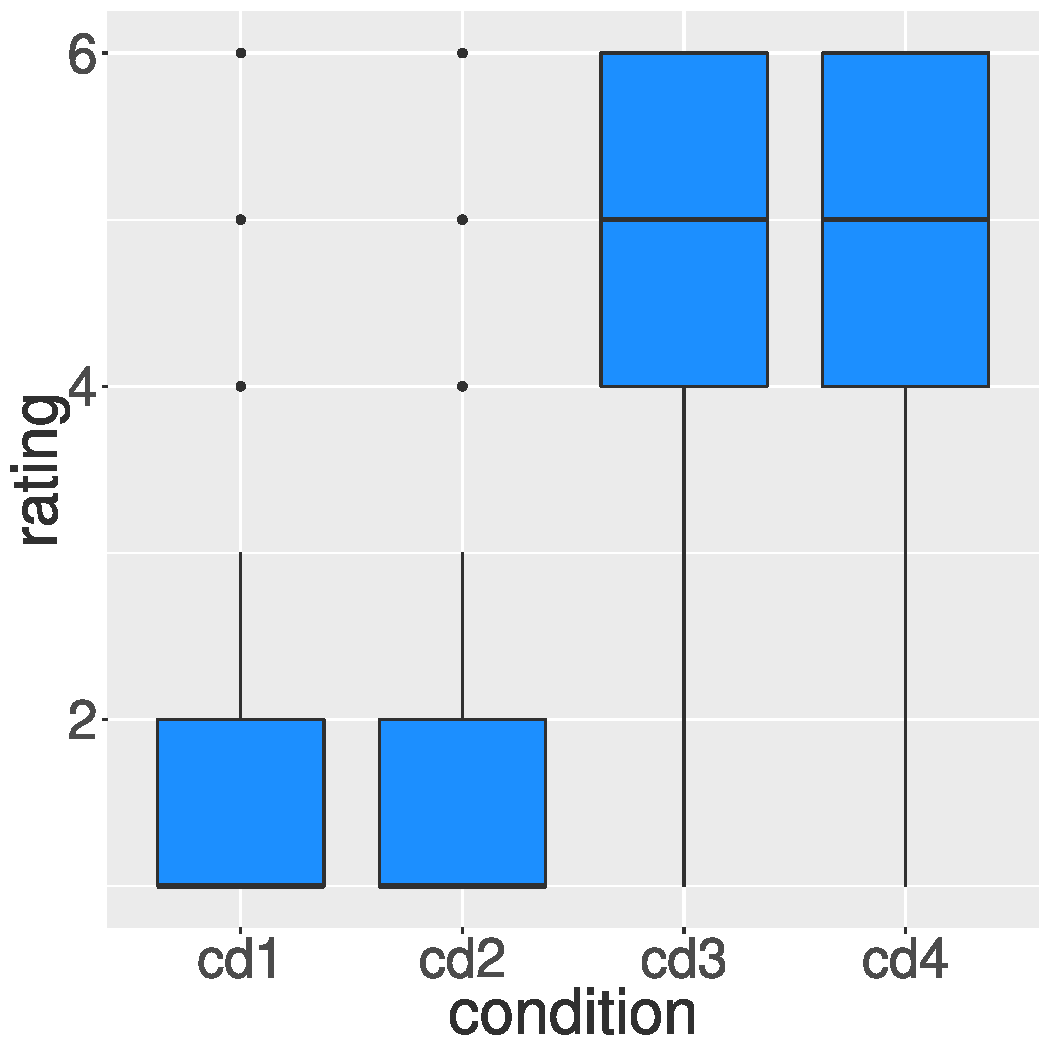
\includegraphics[width=0.85\textwidth]{figures/boxplot.pdf}
    \end{minipage}\begin{minipage}{0.5\textwidth}
        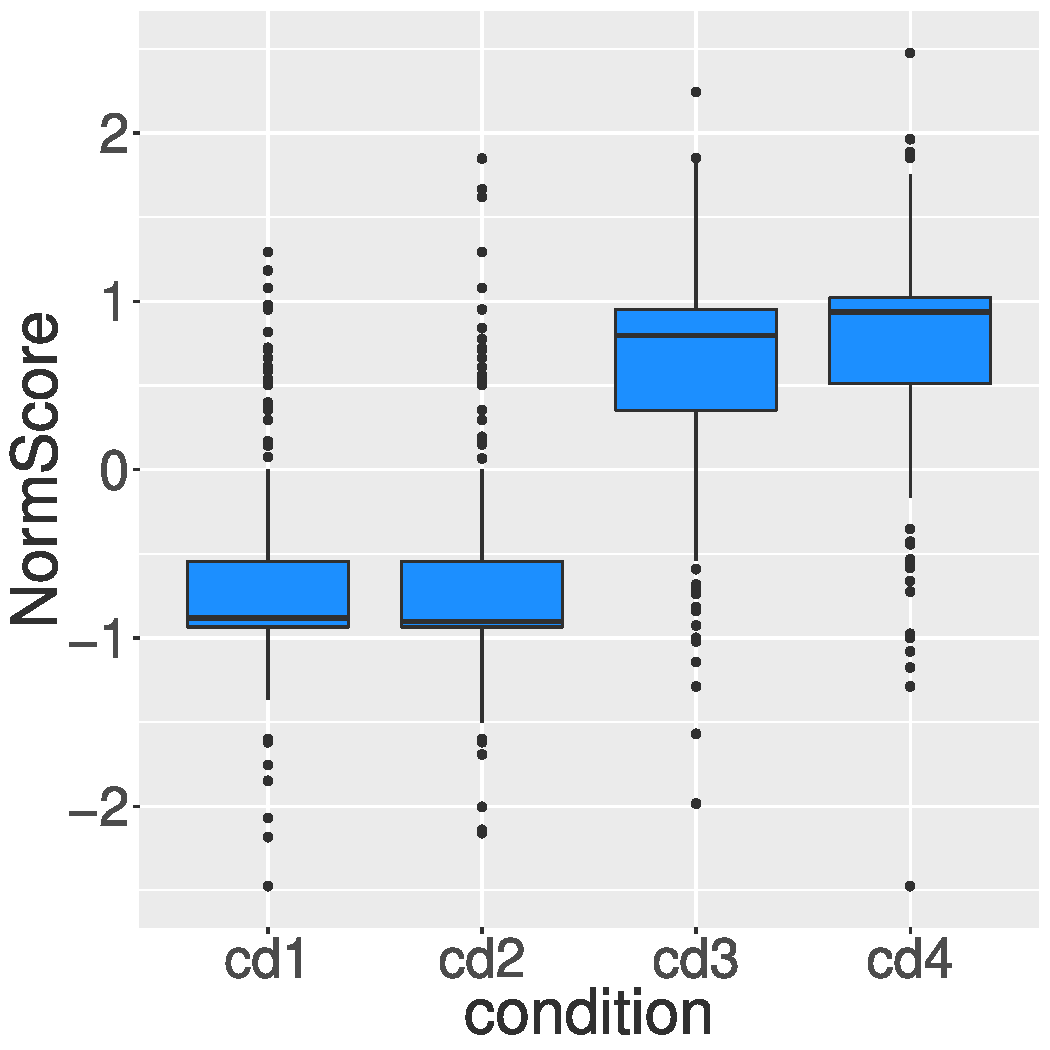
\includegraphics[width=0.85\textwidth]{figures/boxplot_ztrans.pdf}
        \caption{Ratings (left) and norm scores (right) over 4 conditions}
        \label{fig:boxplots}
    \end{minipage}%
\end{figure}

\begin{figure}[p]
    \centering
    \begin{minipage}{0.5\textwidth}
        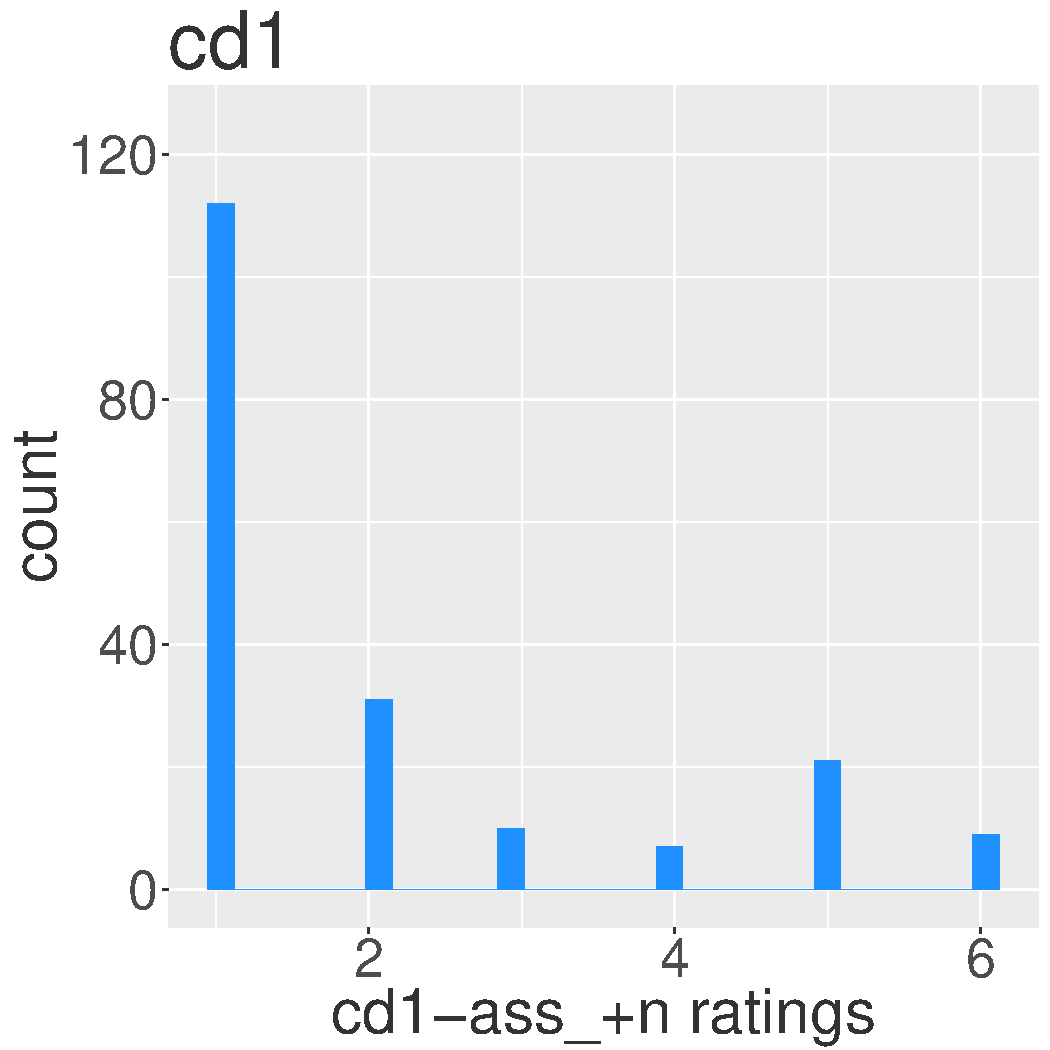
\includegraphics[width=0.85\textwidth]{figures/cd1_hg.pdf}
    \end{minipage}\begin{minipage}{0.495\textwidth}
        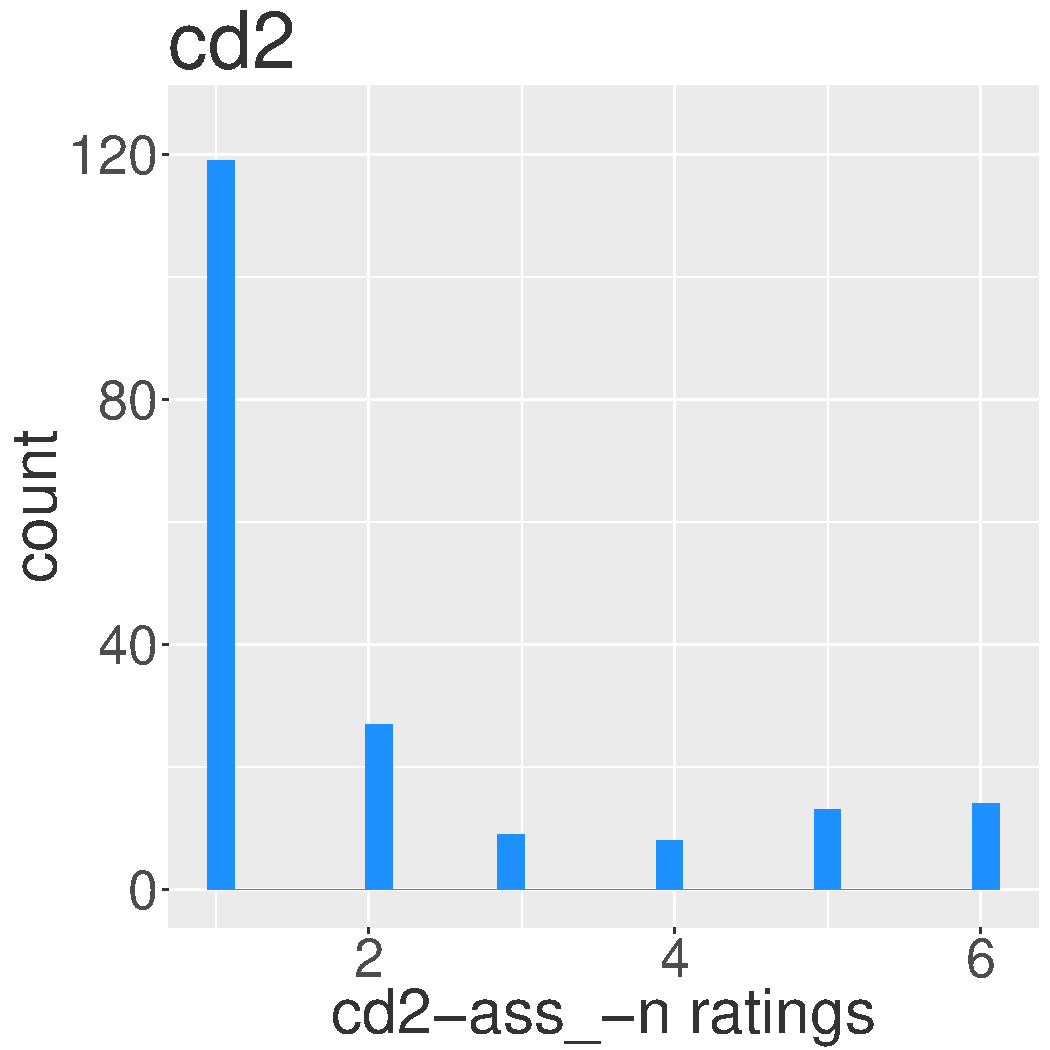
\includegraphics[width=0.85\textwidth]{figures/cd2_hg.pdf}
    \end{minipage}

    \begin{minipage}{0.5\textwidth}
        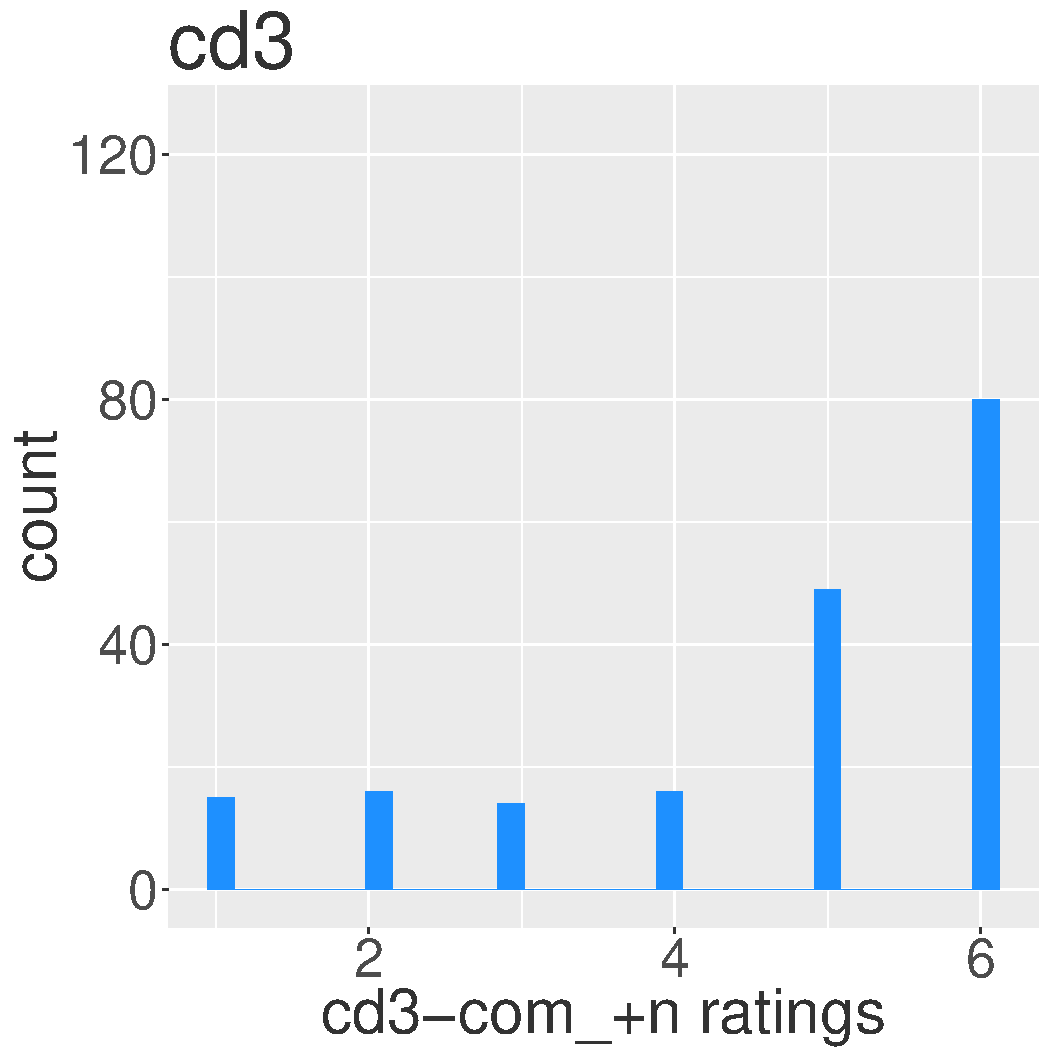
\includegraphics[width=0.85\textwidth]{figures/cd3_hg.pdf}
    \end{minipage}\begin{minipage}{0.5\textwidth}
        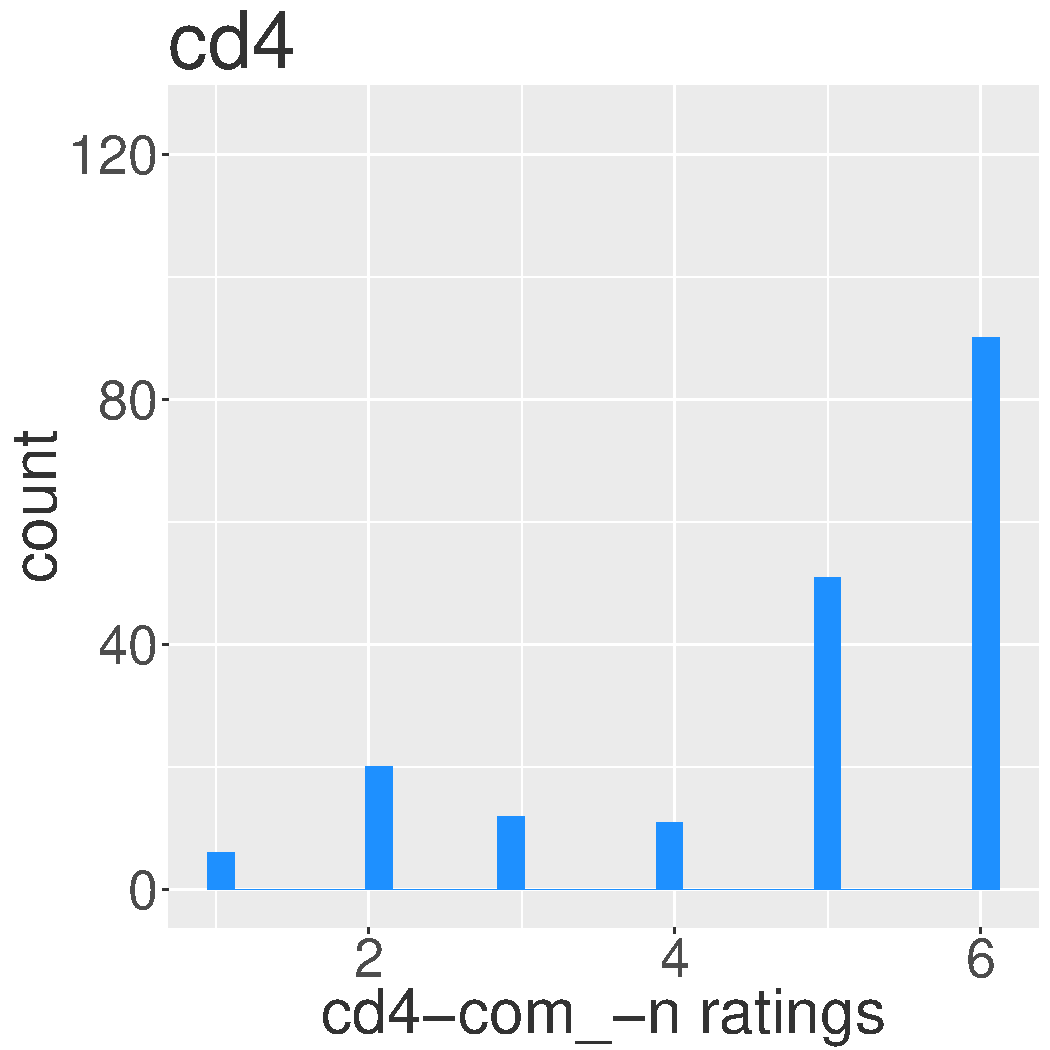
\includegraphics[width=0.85\textwidth]{figures/cd4_hg.pdf}
        \caption{Histograms of 4 conditions (2 factors, 2 levels each)}
        \label{fig:histograms}
    \end{minipage}%
\end{figure}

\subsubsection{Linear mixed effect model}\label{sect_non-parametrics}

I built linear mixed effects models for my data with R \citep{Rsoftware}\footnote{R version 3.6.0 (2019-04-26)} with the lme4-package\footnote{lme4 version 1.1-12} \citep{lme4}. The ratings (1--6) were z-transformed into norm scores. That is, for every participant I calculated means (part\_mean) and standard deviations (part\_sd) and then for all eight ratings per participant (cf. \figref{fig:boxplots} for boxplots of ratings and normscores):

\ea $\text{norm score} = \frac{\text{rating} - \text{part\_sd}}{\text{part\_mean}}$\z

For the further discussion on statistic modelling, the terms \textit{norm score} and \textit{score} will be used synonymously. For model 1, score is taken as a function of an interaction of the fixed effects (factor 1: assertion of \textit{x is tall} (level 1) or not (level 2); factor 2: \textit{noch} absent (level 1) or present (level 2)) and model 2 is a reduced version of model 1, i.e. without the interaction as in model\_1. Both models accounts for participants and contexts as random effects assigning random intercepts. I was able to also include random slopes for both factors correlated with the respective two random intercepts, resulting in a maximally random effects structure for my models. Find the outline of the basic structure for model 1 in \REF{LME_model_1} and for model 2 in \REF{LME_model_2}:

\ea score \textasciitilde fac.1 $*$ fac.2 + (1 + fac.1 $*$ fac.2 | partcpt.) + (1 + fac.1 $*$ fac.2 | context) + $\varepsilon$ \label{LME_model_1}     
\ex score \textasciitilde fac.1 + fac.2 + (1 + fac.1 $*$ fac.2 | partcpt.) + (1 + fac.1 $*$ fac.2 | context) + $\varepsilon$ \label{LME_model_2}        \z

Find the outpout for model 1 in \tabref{R_output_model_1}. Note that I used the lmerTest package\footnote{lmerTest version 3.1-0} \citep{lmerTest} to add $p$-values to the lmer-summary.


\begin{table}
\resizebox{\linewidth}{!}{%
\begin{tabular}{lS[table-format=-1.5]S[table-format=1.5]S[table-format=2.5]S[table-format=-2.3]S[table-format=<1.1e3,table-align-exponent
=false]l}
\lsptoprule
Fixed effects:    & {Estimate} & {Std. Error} & {df}        & {$t$ value}   & {Pr(>|t|)}  & \\\midrule
\texttt{(Interecept)}        & -0.65142 & 0.05822 & 46.21000 & -11.190  & 9.5e-15   & {***}\\
\texttt{fac\_1com}           & 1.36396  & 0.08936 & 45.32000 & 15.264   & <2e-16   & {***}\\
\texttt{fac\_2+n}            & -0.01899 & 0.08184 & 21.78000 & -0.232   & 0.819     & \\
\texttt{fac\_1com:fac\_2+n}  & -0.09008 & 0.10438 & 17.99000 & -0.863   & 0.399     & \\\lspbottomrule
\end{tabular}}
\caption{R output for \texttt{lmer()} call on model 1 \REF{LME_model_1}}
\label{R_output_model_1}
\end{table}

\noindent Factor 1, level 2 has a significant effect with a $t$-value at 15.264 and a $p$-value below \num{2e-16}. Most importantly, there is no significant effect of factor 2, level 2 with a $p$-value of 0.819, cf. \tabref{R_output_model_1}. Moreover, there is not interaction between factor 1, level 2 and factor 2, level 2. To be sure and test specifically for an interaction between factors 1 and 2 I calculated model 2. Comparing models 1 and 2 (in R with \texttt{anova()}) gives the output in \tabref{R_output_anova_model_1_and_2} \citep[cf.][]{winter2013}.

\begin{table}
\resizebox{\linewidth}{!}{%
\begin{tabular}{lrrrrrrrr}
\lsptoprule
                    & {DF} & {AIC}    & {BIC}    & {logLik}  & {deviance} & {Chisq Chi} & {df} & {Pr(>chisq)} \\\midrule
\texttt{mymodel 2}  & {24} & {1467.2} & {1577.8} & {\textminus709.58} & {1419.2}   &               &        &                \\
\texttt{mymodel 1}  & {25} & {1468.4} & {1583.7} & {\textminus709.20} & {1418.4}   & {0.7649}    & {1}  & {0.3818}     \\\lspbottomrule
\caption{R output for \texttt{anova()} call on models 1 and 2}
\label{R_output_anova_model_1_and_2}
\end{tabular}}
\end{table}

Model 2 has a slightly lower AIC and in the comparison of the two models the difference comes out as not significant. This suggests that there is no interaction between factors 1 and 2 ($\chi^{2}(1)=0.7649, p=0.3818$). There is an online repository\footnote{\url{https://github.com/M-K-G/noch_FoDS2}} containing the experimental data and statistics scripts.

\subsection{Conclusions}
At first glance, the results seem to support \citeauthor{umbach2009a_comp}'s \citeyearpar{umbach2009a_comp} analysis. It seems that the non-asserted proposition, i.e. that the standard term of comparison in a \textit{noch}-comparative exceeds a contextually given standard degree, can be canceled and may, therefore, not be regarded presuppositional.

As pointed out by an anonymous reviewer, there may be flaws inherent to the experimental design to the effect that, in line with \citeauthor{Hofstetter2013}'s analysis, the PSP of \textit{noch} in condition 3 is unmet, remains non-accommodated and nothing should be there to contradict/cancel by the continuation. Among other things, it was exactly this point that we attempted to address by asking participants to judge the compatibility of the truth of two sentences. Nevertheless, the issue may remain.\largerpage

A few of the desiderata in retrospect is the lack of judgments for data like \citeauthor{Hofstetter2013}'s \REF{hofstetter_ABER_peter_nicht_gross} (repeated here as \ref{hofstetter_ABER_peter_nicht_gross_2}). What is it that makes this sentence seemingly infelicitous and under what circumstance could this sentence be felicitous? Would an antecedent comparison as in \REF{comp_additional_comp_NOCH} (cf. conditions 3 and 4 above) make \REF{hofstetter_ABER_peter_nicht_gross_2} felicitous? It is possible -- in this instance I do not have reliable introspective judgments and conclude that more experimental work is required taking a different approach in eliciting judgments. %\footnote{ With regard to the translation in \REF{comp_additional_comp_NOCH}, as far I was able to determine \textit{still} in postposition might be the preferred option for native speakers of American English. Potentially interesting for the current proposal is the observation that relying on \textit{even} for the translation here would more strongly suggest that the standard term of comparison exceeds a contextual standard with \REF{still_taller} being felicitous and \REF{even_taller} infelicitous.

%\ex. Peter is taller than Kurt. Paul is still taller than Peter but Peter is not tall. \label{still_taller}

%\ex. *Peter is taller than Kurt. Paul is even taller than Peter but Peter is not tall. \label{even_taller}

%Whether this is indeed the case needs to be tested of course. In turn, this difference between \textit{even} and \textit{still} might pattern BLA BLA. Diachronic and experimental work on \textit{even} as well as German \textit{sogar} (`even') would elucidate this issue.}

\ea (Adapted from \citealt[p. 27, ex. 2/49]{Hofstetter2013})\\
\gll * Paul ist noch größer als Peter, aber Peter ist nicht groß.\\
     {} Paul is still tall.COMP than Peter but Peter is not tall\\ \label{hofstetter_ABER_peter_nicht_gross_2}

\ex[?]{\gll Peter ist größer als Kurt. Paul ist noch größer als Peter, aber Peter ist nicht groß.\\
       Peter is tall.COMP than Kurt Paul is still tall.COMP than Peter but Peter is not tall\\
\glt   `Peter is taller than Kurt. Paul is still taller than Peter but Peter is not tall.' \label{comp_additional_comp_NOCH}}
\z
With these caveats in mind, and accepting the results of the above experiment, I will turn back to the semantics of \textit{noch} in the next section.

\section{Updating the semantics of \textit{noch}\textsubscript{comp}}\label{sec_semantics_update}

Based on the above findings, I propose to update the lexical entry for \textit{noch}\textsubscript{comp}:

\ea\relax \(
   ⟦\text{noch\textsubscript{comp}}⟧ = 
   \lambda \text{d*} \in \text{D}_{\text{d}} \text{.} 
   \lambda \textsc{Co} \in \text{D}_{\langle\langle \text{d} , \text{t} \rangle , \langle \langle \text{d} , \text{t} \rangle , \text{t}\rangle\rangle} \text{.} 
   \lambda \text{D}_{1} \in \text{D}_{\langle \text{d} , \text{t} \rangle } \text{.}
   \lambda\text{D}_{2}\in \text{D}_{\langle \text{d},\text{t}\rangle}: \text{d*} \leq \text{max}(\text{D}_1)
\). \textsc{CO} max(D$_1$) max(D$_2$),\\
where d* is a free variable to be bound by the context and ranked lower than the max-degree of the comparison base 
and \textsc{Co} is the comparative operator of the \textit{noch}-comparison. \label{noch_comp_entry} \z

I assume clausal comparison with the comparison operator of type \citep[cf.][]{Beck2011}: 
    \[\langle\langle \text{d},\text{t}\rangle,\langle\langle \text{d},\text{t}\rangle,\text{t}\rangle\rangle \] 
and the lexical entry in \REF{comp-operator}. The logical form for sentence \REF{B_noch_>_Adam} (=\ref{umbach_21}) is in \REF{LF_B_noch_>_Adam} where one can see that quantifier raising solves the problem of the type mismatch of the DegP and adjective (for both clauses). Via predicate abstraction in \REF{PA_on_clauses} and intermediate steps in \REF{calc_plugin} (relying on the lexical entry \ref{comp-operator}), the LF in \REF{LF_B_noch_>_Adam} yields \REF{output_calc} (relying on the lexical entry for \textit{noch} in \ref{noch_comp_entry}), cf. LF in \figref{fig:LF_B_noch_>_Adam}.

\ea\relax $⟦$-er$⟧$ = $\lambda$D1.$\lambda$D2. max(D2) $>$ max(D1) \label{comp-operator}

\ex\ea \textit{Berta ist noch größer als Adam.} \label{B_noch_>_Adam}
\ex\relax [ noch d* [-er than [2[Adam ist [AP t2 groß]]] [1 [ Berta ist [AP t1 groß]]]]] \label{LF_B_noch_>_Adam}
\z
\ex\ea \label{PA_on_clauses}\relax [1 [ Berta ist [AP t1 groß]]] = $\lambda$d. B is d-tall
\ex\relax [2 [Adam ist [AP t2 groß]]] =  $\lambda$d. A is d-tall \z
\ex\relax [ noch d* [$\lambda$D1.$\lambda$D2. max($\lambda$d. B is d-tall) $>$ max($\lambda$d$'$. A is d$'$-tall) ]] \label{calc_plugin}
\ex $\lambda$d*.$\lambda$D$_1$.$\lambda$D$_2$: d*$\leq$max($\lambda$d. A is d-tall). max($\lambda$d. A is d-tall)$<$ max($\lambda$d. B is d-tall)  \label{output_calc}
\ex \REF{B_noch_>_Adam} is defined only if Adam is taller than something else relevant, i.e. the degree d*, provided by the context, and it is true if and only if Berta is taller than Adam.\z

\begin{figure}
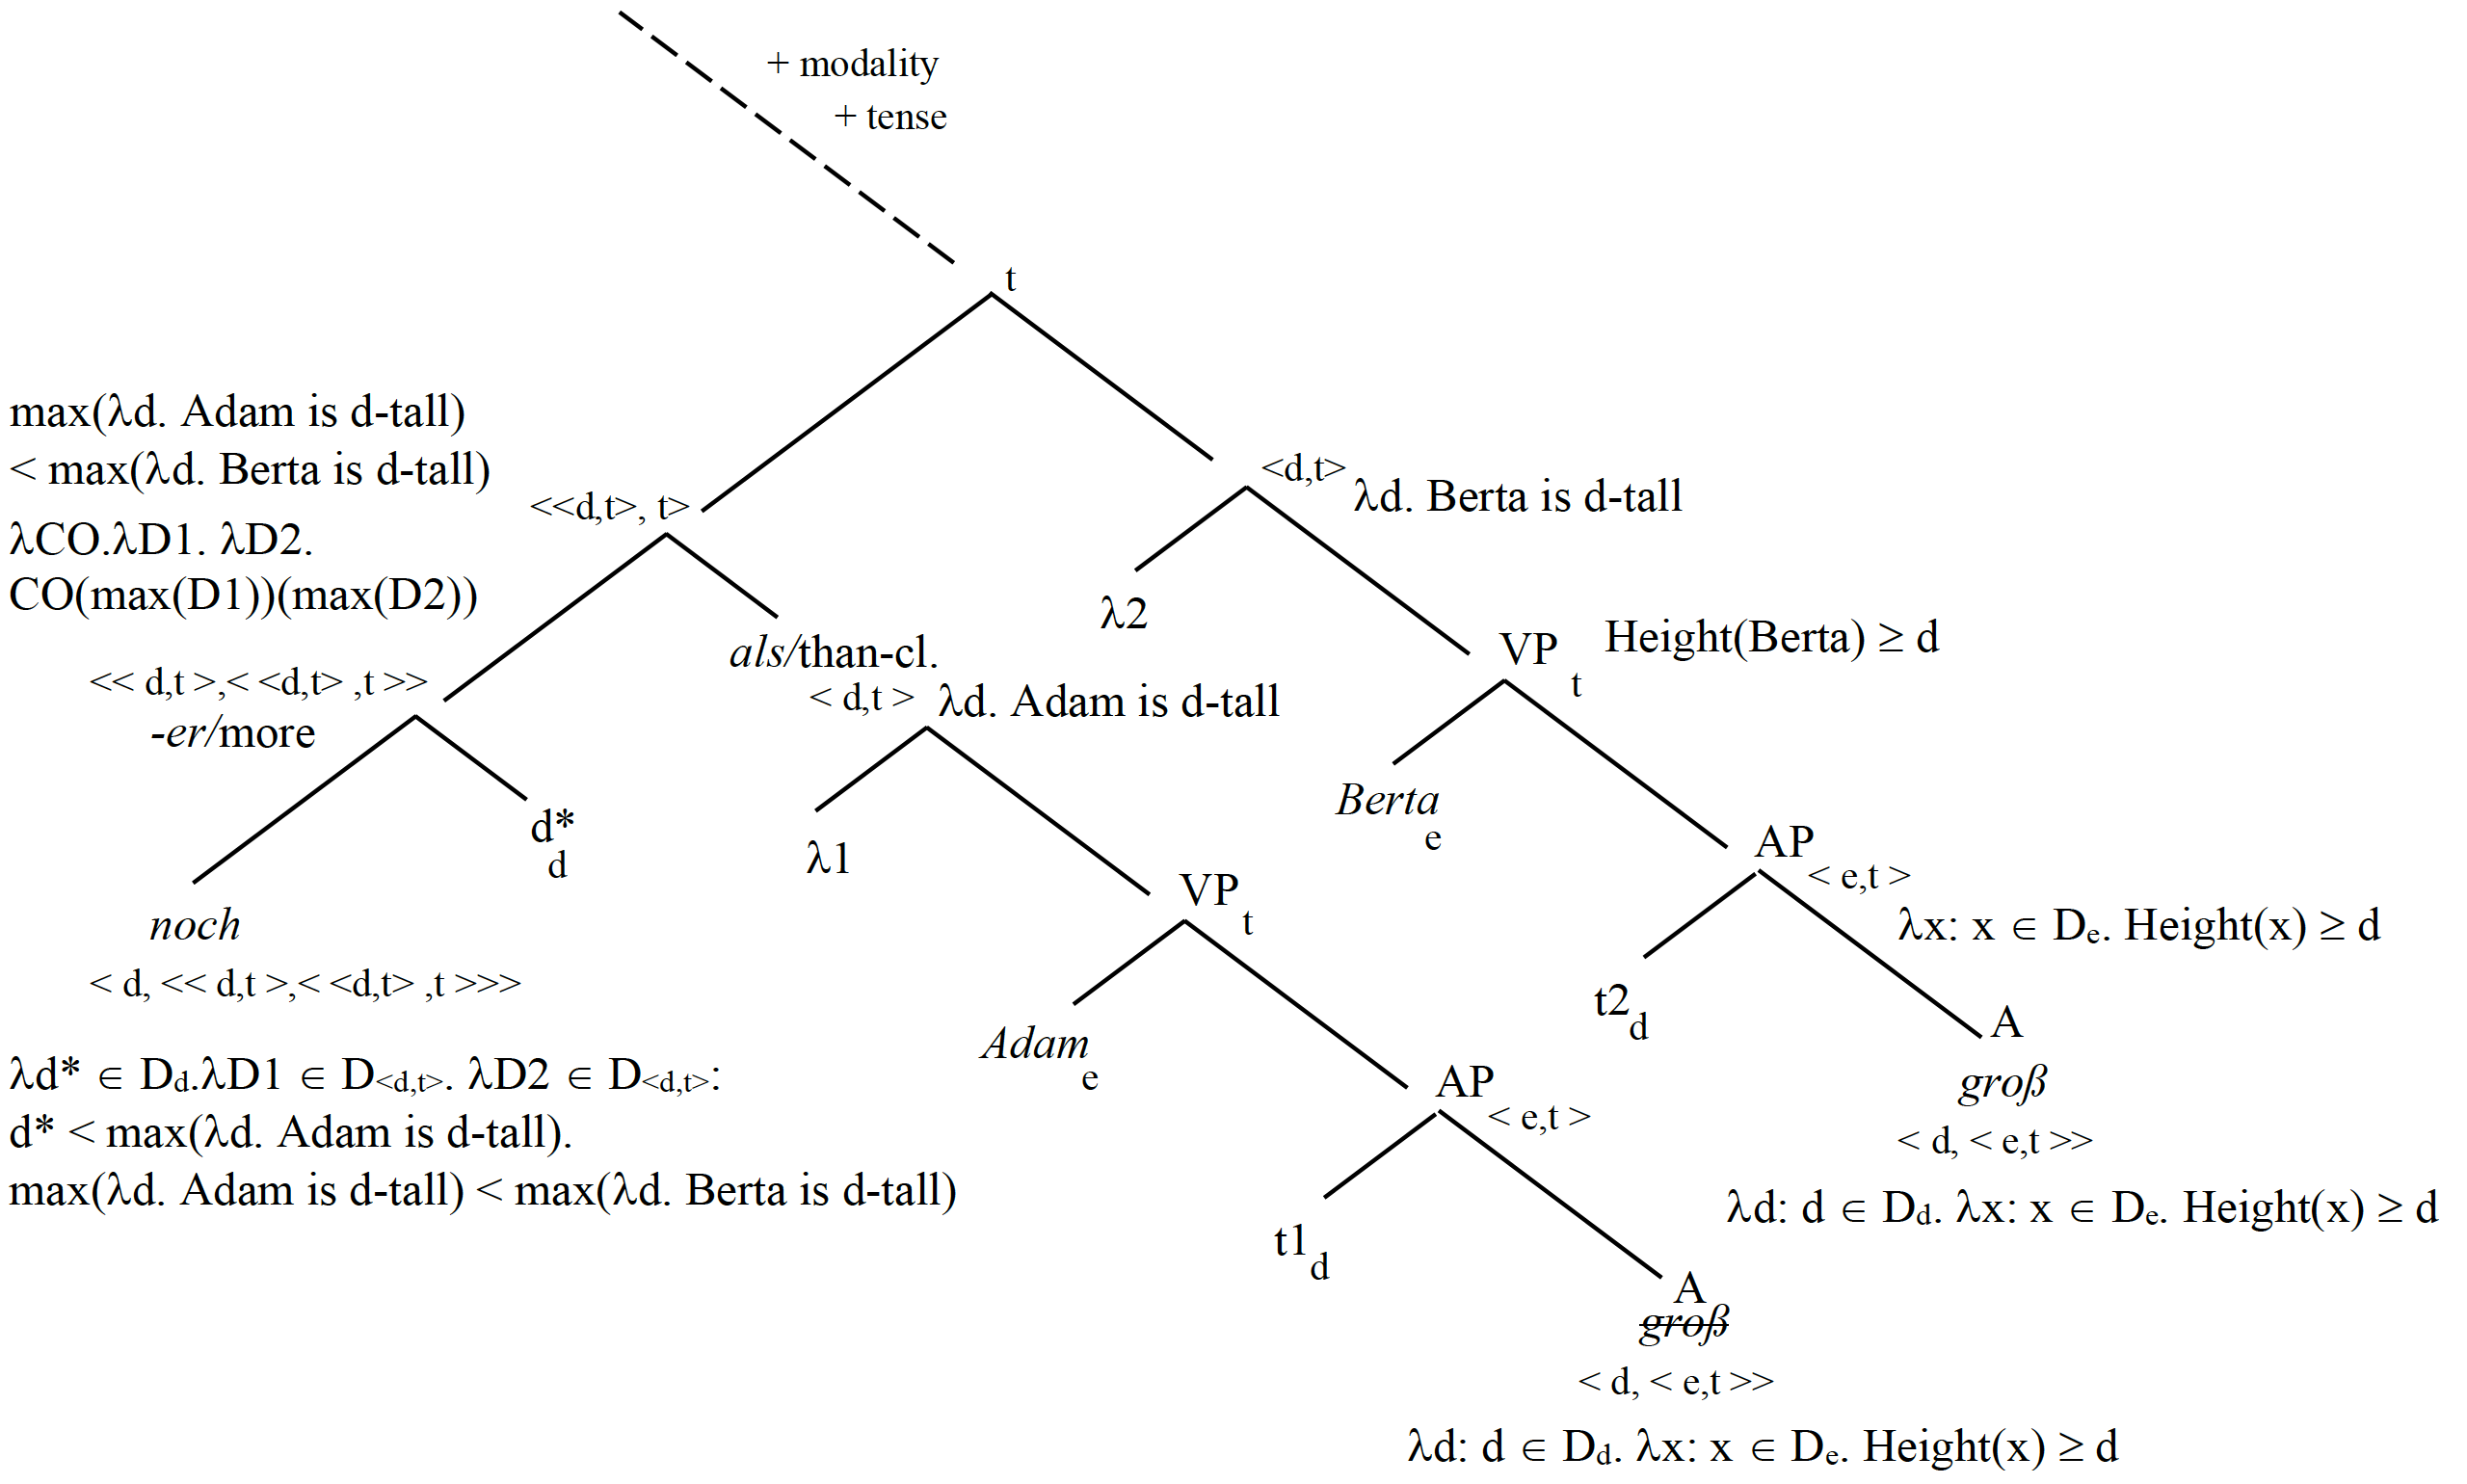
\includegraphics[width=1\textwidth]{figures/LF-mod_comp}
\caption{LF for \REF{B_noch_>_Adam}}
\label{fig:LF_B_noch_>_Adam}
\end{figure}

\noindent There is no condition on the context that Adam is taller than a contextually given standard. Thus, norm relatedness does not arise (cf. \citealt{umbach2009a_comp} and \sectref{SubSec_umbach_analysis}), which seems to be the desired situation given the experiment reported above. In essence, the free degree variable \textit{d*} is what norm relatedness hinges on. Depending on what in the context d* refers to, \textit{noch} will give rise to norm relatedness. Let's assume the context provides a proposition along the lines of condition 1 (cf. \tabref{tab:4_conds}, page \pageref{tab:4_conds}), e.g. \textit{Adam ist groß} (`Adam is tall') preceding \REF{B_noch_>_Adam}. In such a case, the maximum degree to which \textit{Adam is tall} (i.e. comparison base of \textit{noch}-comparative) is equal or higher than the degree of the height of Adam as per the proposition from the context -- which comes with a positive operator and puts Adam's height above a standard of height. \citeauthor{umbach2009a_comp} \citeyearpar{umbach2009a_comp} points to this aspect of meaning of positive degree adjectives in the context of \textit{noch}\textsubscript{comp}. So do, more generally, \citet{vonStechow1984,stechow2006} and \citet{Beck2011}: the idea is that there is a scale \textit{S} introduced by an adjective, e.g. tall, and there is a function \textit{N} that yields the neutral part of the scale and the neutral part \textit{N(S)} contains all elements that are neutral in terms of tallness. The positive operator universally quantifies over all the degrees contained in the neutral part of the scale \citep{stechow2006}.

\ea (Adapted from \citealt[ex. 3-1--3-3]{stechow2006})\\ S\hspace{15pt}|{-}{-}{-}{-}{-}{-}{-}{-}{[}{-}{-}{-}{-}{-}{-}{-}{-}{-}{-}{-}{-}{-}{-}{-}{-}{-}{-}{-}{]}{-}{-}{-}{-}{-}{-}{-}{-}$\to$|\newline .\hspace{22pt} short \hspace{20pt} Neutral \hspace{25pt} tall
\ex \textit{Adam is tall.}\newline $⟦$\textbf{Pos}\textsubscript{N,S}$⟧$\textsuperscript{g} = $\lambda$A\textsubscript{dt}.(\textbf{$\forall$}d $\in$ N(S)) A(d) 
\ex  The positive operator\newline $⟦$\textbf{Pos}\textsubscript{N,S}$\lambda$d.tall\textsubscript{S}(d)(Adam)$⟧$ iff ($\forall$d $\in$ N(S)) HEIGHT(Adam) $\geq$ (d)\newline|{-}{-}{-}{-}{-}{-}{-}{-}{[}{-}{-}{-}{-}{-}{-}{-}{-}{-}{-}{-}{-}{-}{-}{-}{-}{-}{-}{-}{]}{-}{-}{-}{-}{E}{-}{-}{-}$\to$|\z

With regard to the semantics of \textit{noch}, if there is no such proposition in the context but e.g. a comparison as in condition 3 (cf. \tabref{tab:4_conds}, p. \pageref{tab:4_conds}), then there is no Pos-operator involved \citep[62]{vonStechow1984} and, in \citeauthor{umbach2009a_comp}'s words, norm-relatedness does not arise.

\ea \itshape Berta ist noch größer als Adam. \label{B_noch_>_Adam_repeat}\z

The question that has remained unanswered is what happens in out-of-the-blue \textit{noch}-comparatives -- with no overt antecedent. \citeauthor{umbach2009a_comp} argues that for \REF{B_noch_>_Adam} (repeated here as \REF{B_noch_>_Adam_repeat}) an antecedent gets accommodated as being ``composed out of the comparison base of the \textit{noch} comparative and the norm of the adjective (with respect to the comparison class)'' \citep[10]{umbach2009a_comp}. Essentially, this accommodated antecedent is of the form `Adam is tall', i.e. it features \citeauthor{stechow2006}'s \citeyearpar{stechow2006} Pos-operator.


\section{Diachronic data}\label{sec_diachronic_data}


The following discussion mainly relies on data from the DDD corpora of Old German (OG, \citealt{ddd_OG}) via ANNIS \citep{annis_og}. Other supplementary sources include \citet{kali}, and the TITUS project \citep{titus}.

The OG period was split into subperiods: 

\begin{description}[style=unboxed,font=\normalfont\itshape,noitemsep]
\item[OG0] pre-750 
\item[OG1] 750--850 
\item[OG2] 850--950 
\item[OG3] 950--1050
\end{description}

The existing part-of-speech (POS) annotation was supplemented with annotations specifically geared towards occurrences of \textit{noh}, the OG form of ModGerman \textit{noch} (in the following, I will use the two forms interchangeably). The existing (DDD) POS tags for \textit{noh} are ADV (adverbial) and KON (conjunctive). For this paper, I ignore conjunctive uses of \textit{noh} such as in \REF{KON_noch}. The ADV occurrences of \textit{noh} were -- on top of the existing annotation -- annotated for temporal, additive and comparative uses, i.e. \textit{noch}\textsubscript{temp}, \textit{noch}\textsubscript{add}, and \textit{noch}\textsubscript{comp}.


\ea\gll Nist thes gisceid \textbf{noh} giuuant, uuio er girrit thaz lant, uuio er iz allaz uuirrit, ioh thesa uuorolt merrit.\label{KON_noch}\\
       Not-is of.this boundary \textbf{nor} measure, how he confuses the land, how he it all stirs, and this world injures.\\
\glt   {`There is neither boundary nor measure to which he disturbs the country as he causes it trouble and to the entire world.'} \\ \hfill (Otfried DDD\_O\_Otfr.Ev.4.20, edition 278--289 via ANNIS) % 1.OG2.OtfEbKell.281.27
\z

\tabref{tab:overview_subperiods_and_sources} gives an overview of occurrences of \textit{noh\slash noch} in the diachronic data available in the DDD corpus. \tabref{tab:frequencies_of_noh} shows the frequencies of all occurrences of adverbial uses of \textit{noh} across the subperiods OG1--OG3 in all of the text of the DDD corpus.


\begin{table}[p]
\begin{tabular}{llrr}
\lsptoprule
{OG1:} & {form} & {KON} & {ADV}  \\
\midrule
Tatian: & prose & 95 & 43  \\
Isidor: & prose & 11 & 9 \\
Monsee Fragments: & prose & 8 & 4 \\
Heliand: & verse & 2 & 36 \\ % Heliand - maybe exclude by suggestion of reviewer 1
Old Saxon Genesis: & verse & 0 & 5 \\
\midrule
{OG2:} & {form} & {KON} & {ADV}  \\
\midrule
Otfried: & verse & 51 & 72 \\
Smaller OG language monuments & (mix.) & 100 & 12 \\
\midrule
{OG3:} & {form} & {KON} & {ADV}  \\
\midrule
Notker (various) & prose & 96 & 118 \\
\lspbottomrule
\end{tabular}
\caption{Subperiods and sources; KON vs. ADV\label{tab:overview_subperiods_and_sources}}
\end{table}

\begin{table}[p]
\begin{tabular}{ll}
\lsptoprule
subperiod	& freq. (\%)	\\
\midrule
OG1		& 0.073 \\
OG2		& 0.088 \\
OG3		& 0.070\footnote{The frequency for OG3 is is an approximation since the corpora's word counts include the parts in Latin.}\\
\lspbottomrule
\end{tabular}
\caption{Frequencies of \textit{noh} (ADV), based on no. of tokens in OG subperiods}
\label{tab:frequencies_of_noh}
\end{table}

Regarding OG1, the Heliand text had to be excluded since its periodisation is unclear with two different sources having found their way into the corpus texts.

Otfried is the only major text available from OG2 (and unfortunately in verse) and, therefore, was included. The additional material available from OG2 are minor hits from the \textit{Smaller Old High German language monuments} (`Kleinere Althochdeutsche Sprachdenkmäler') which, in turn, are difficult to pin down in terms of periodisation as a whole. Hits from single texts were considered for annotation. The numbers in \tabref{tab:subperiods_and_readings} are based on the final selection of corpus text considered.


\begin{table}[p]
\begin{tabular}{lcccc}
\lsptoprule
	& (cjn) & temp (amb.)\footnote{read as e.g.: in OG2, 2 \textit{noh} are comparative, out of which (2) are ambiguous to other readings}& comp (amb.)	& add (amb.)	\\
\midrule
OG1		& (122) & 45 (8)    & 1 (1/0?)  & 12 (4)    \\
OG2		& (66)  & 53 (6)    & 2 (2)     & 8 (6)     \\
OG3		& (54)  & 21 (4)    & 3 (0)     & 4 (4)     \\
\lspbottomrule
\end{tabular}
\caption{Subperiods and readings of \textit{noh}.}
\label{tab:subperiods_and_readings}
\end{table}

A full annotation of 214 tokens from the OG3 (Notker) texts is incomplete as of yet. The numbers in the above table are based on 76 OG3-tokens annotated in detail and are to be taken to be representative for the entire subperiod. Among the 76 tokens categorized, there was one \textit{noh} with an unambiguously comparative reading. The annotation of 76 tokens was supplemented with targeted corpus searches for \textit{no(c)h}\textsubscript{comp} uses, with various queries among all 214 uses of \textit{noh} in the Notker texts which yielded two more hits of \textit{no(c)h}\textsubscript{comp}, bringing the total for OG3 to 78 tokens.

In the following, I want to discuss the most important aspects and examples of the diachronic data. The most problematic bit of diachronic data is \REF{OG1_comp?_00}:

\ea\gll Ibu auuar in aftrun steti {ga sizzis} enti quuimit dir otlihhero {qui dit} daer dih za demo {naht muose} {la dota,} sizzi.2SG.IMP NOH hohoro.COMP baz.COMP enti ist dir danne {guot lihhora;}\\
       If but in back place you.sit, and comes you `lower', says, who you to the dinner invited, sit still/even higher better, and is you then honorable\\
\glt   {`But if you sit down somewhere in the less prominent places and the person who invited you for dinner tells you to sit in a more prominent place, then it is better to sit still higher and that is then honorable.'} \label{OG1_comp?_00} \\ \hfill (MonsF-1,M.XIV, edition 141--152)
\z


\REF{OG1_comp?_00} is problematic for a number of reasons. The most striking problem is that it could be a very early instance of \textit{noh}\textsubscript{comp}. Example \REF{OG1_comp?_00} is the reason that, in \tabref{tab:subperiods_and_readings},\footnote{These numbers do not straight forwardly match numbers in \tabref{tab:overview_subperiods_and_sources} since they account for ambiguities, only show \textit{noch} labelled as ADV, and are based on a smaller set of texts.} the first line for \textit{noh}\textsubscript{comp} shows 1 (1/0?). Let us look at it in more detail: the wider context is about humility and humbleness. \REF{OG1_comp?_00} is part of an allegory and the allegorical context is limited in potential to disambiguate. The preceding context talks about how shameful it is to take a prominent seat at a table when invited to dinner and then being told to take a less prominent seat.

The comparative reading doesn't have strong support as the expected action to attain humility (in a Christian world view) would be to turn down an offer to sit higher/take a more prominent seat. A temporal (further-to) interpretation runs into the problem that this is a hypothetical situation and there is no detectable temporal sequence aside from the salient time of mentioning. Moreover, in contrast to the majority of early uses of \textit{noch}, it lacks a temporal particle adjacent to it. A conjunctive, coordinating interpretation would require another negative constituent to be coordinated with. The example is from the Mondsee Fragments, it is in Bavarian dialect and dates from the early 9th century (\textasciitilde 810AD) \citep{annis_og}. Thus, if \REF{OG1_comp?_00} constitutes an instance of \textit{noch}\textsubscript{comp}, it would (i) indicate that Southern dialects of German might have been more innovative and (ii) mean that the comparative reading has been available relatively soon.

Let us turn to more examples of diachronic data, especially ones ambiguous between temporal and comparative readings (both \ref{OG2_noch_blind_man} and \ref{OG2_noch_mehr_ruehren_first} are from Otfrid, OG2):

\ea\gll Ladotun auur tho then man, ther thes gisiunes biquam, quadun, sih thera.GEN dati.GEN noh tho baz biknati.SUBJ.PAST.3.SG.\\
       invited but then the man, who of.the seeing became, said, himself of.the deed still/even there better appraise.\\
\glt   {`They then requested of the man who gained eyesight to appraise/evaluate his action still/even there more thoroughly.'}\label{OG2_noch_blind_man} \\ \hfill (1.OG2.OtfEbKell.202.105)
\z
The context for \REF{OG2_noch_blind_man} is a story of Jesus giving a blind man eyesight. The miracle was worked on a Sabbath, which is the reason for public outcry. The formerly blind man is being questioned by the people and by the local high council about the events and about his opinion of Jesus -- for the third time in \REF{OG2_noch_blind_man}. The criticism Jesus faces is rooted not only in breaking Sabbath but more importantly that he claims to be god's son, which, in turn, allowed him to do as he wished on a Sabbath.

This sentence is ambiguous to a temporal and a comparative reading. Both, the PSPs for the temporal and the comparative interpretations are satisfied in the context. The preceding context features two instances of the formerly blind man stating his opinion of Jesus. Moreover, there is a (locative/temporal cf. e.g. \citealt{petrova2011}) particle adjacent to \textit{noh}. The comparative interpretation is supported by the fact, that the man has stated his opinion of Jesus twice before and, moreover, the statements regarding Jesus have changed in degree (`to the better') -- in the eye of the public: at first, the man called Jesus `the savior'; at the second time, he called him `a friend of god ... a divine prophet'. Thus, he lessened the degree to which Jesus was stated to be akin to god. Another argument for a comparative interpretation is that, arguably, the finite verb \textit{biknati} (\textit{biknaen}, `to confess, appraise, declare') is an atelic verb (`hold a belief/attitude') rather than an accomplishment (`declare your attitude/make a statement'). The lack of a direct (accusative) object would support that view. In conclusion, I argue that the comparative interpretation is salient.

As noted, \REF{OG2_noch_mehr_ruehren_first} is ambiguous to a temporal and a comparative reading:

\ea\gll Thar uuarun mit githuinge thie iungoron noh tho inne, sie scolta ruaren NOH tho mer thaz selba uuoroltlicha ser.\\
       There were with violence the apostles still there inside, they should move still/even there more the same earthly suffering.\\
\glt   {`The apostles were still inside with violence, they should continue to move/stir the earthly suffering.'}\label{OG2_noch_mehr_ruehren_first} \hfill (1.OG2.OtfEbKell.351.12)
\z
The example in \REF{OG2_noch_mehr_ruehren_first} is set in the context of an allegory with the apostles fishing on -- and Jesus on the shores of -- the lake Sea of Galilee. The story states that Jesus is not with the apostles anymore and they now have to continue their work without him. Thus, they are situated in the rough waters of the lake (=\,out in the world) whereas Jesus is on the calm and dry shore (=\,dead; in heaven). \REF{OG2_noch_mehr_ruehren_first} is ambiguous to a temporal and comparative reading. I will discuss it in more detail in the following section.

The following bits of data can be straightforwardly interpreted as comparative uses of \textit{noch}. They all date from the OG3 period, indicating that during this time (950--1050) the comparative reading of \textit{noh} is available.

\ea\gll Úbe árg uuéllen uuêlih íst, árg kemúgen, dáz íst nóh uuêlichera.\\
       if evil.ACC to.want bad is, evil be.able.to.do, that is still/even worse.\\% http://www.kali.uni-hannover.de/glosse.php?txt=7&seite=60
\glt   {`If it is bad to want evil things, then to be able to do evil things is still/even worse.'}\label{OG3_noch_schlimmer} \hfill (Notker.Boeth-DeConPhil.III.201)
\z
\REF{OG3_noch_schlimmer} is unambiguously comparative. There is no temporal sequence available and there is no temporal particle adjacent to \textit{noh}. In the comparative interpretation, the comparison base (wanting evil) is in the same token. Similarly, there is no temporal sequence discernible in \REF{OG3_noch_wissend}:

\ea\gll Ér íst tero góto {chúnnigosto .} nóh tánne bíst tû {chúnnigora .} uuánda ratio gemág mêr dánne {sermo .}\\
       He is of.the gods most.knowledgeable. Still/even then/there are you more.knowledgeable, because reason can.do more than the.conversation.\\
\glt   {`He is the most knowledgeable about the gods. But you are still/even more knowledgeable because reason can achieve more than conversation.'}\label{OG3_noch_wissend} \\ \hfill  (1.OG3.N:Mart.Cap.II.111-121.J)
\z
There is no temporal sequence that would support a temporal interpretation. While it is odd that the first clause has the superlative form of the adjective \textit{chunnig} (`knowledgeable'), the Latin gloss does not feature superlative, and I assume that the superlative in the OG version is there for rhetorical reasons. The comparative reading is salient -- in both the Latin and the OG versions. In \REF{OG3_noch_more_glory_first} (from OG3) the \textit{noh} is adjacent to \textit{mêrun} (`more'), there is no temporal sequence and \REF{OG3_noch_more_glory_first} can unambiguously be interpreted as comparative:

\ea\gll Michel ist íro guôllichi an dînemo haltâre christo. [Lat.] Ímo selbemo gíbest du noh mêrun guôllichi. unde mêrun ziêreda. sô dû in gesezzest ad dexteram tuam.\\
       Great is her glory in your savior christ. [Lat.] him self give you still/even more glory. and more adornment. as you him set to\_LAT right\_LAT your\_LAT.\\
\glt   {`Great is the glory of the church in your savior christ. You give him still/even more glory and more adornment by setting him at your right side.'}\label{OG3_noch_more_glory_first} \hfill (1.OG3.N:Ps:20.61--63)
\z
The major conclusions to be drawn from the data (\tabref{tab:subperiods_and_readings}) are (i) that the comparative reading of \textit{noch} developed within the OG period and (ii) that the (unambiguously identifiable) additive reading became available alongside the comparative reading. \citeauthor{umbach2009a_comp} \citeyearpar{umbach2009a_comp} stresses that \textit{noch}\textsubscript{comp} shares a number of properties with \textit{noch}\textsubscript{add}, i.e. ``patterns with the additive reading of \textit{noch}'' \citep[9]{umbach2009a_comp}. Moreover, while \citeauthor{beck2016a_sub} does not state so, her \citeyearpar{beck2016a_sub} analyses of the continuative, the subconstituent reading, and the further-to reading of \textit{noch}\textsubscript{temp} seem a convincing trajectory from a ``standard'' continuative reading towards an additive reading. Both, \citeauthor{umbach2009a_comp}'s \citeyearpar{umbach2009a_comp} and \citeauthor{beck2016a_sub}'s \citeyearpar{beck2016a_sub} analyses and views combined make for a compelling argument to assume that \textit{noch}\textsubscript{comp} developed based on \textit{noch}\textsubscript{add}. However, the mere observation that \textit{noch}\textsubscript{comp} shares similarities with \textit{noch}\textsubscript{add} does not justify the assumption that the former is derived from the latter -- those similarities may well be due to the common origin in \textit{noch}\textsubscript{temp}. While the diachronic, empirical basis -- despite considerable efforts -- is admittedly rather weak, I argue that the early ambiguous cases (\textit{noch}\textsubscript{comp} and \textit{noch}\textsubscript{temp}) should weigh more heavily. Both \REF{OG2_noch_blind_man} and \REF{OG2_noch_mehr_ruehren_first} and their contexts license a temporal reading (especially when excluding the comparative operator for the sake of contrasting the involved meaning components as minimal pairs introspectively). The fact that this ambiguity with a temporal interpretation exists among the earliest uses of comparative \textit{noch} in those contexts leads me to propose an analysis of \textit{noch}\textsubscript{comp} being derived from \textit{noch}\textsubscript{temp} in the next section. With regard to example \REF{OG1_comp?_00}, as problematic as it is for the overall timeline I am suggesting, \REF{OG1_comp?_00} could provide support for my proposal as a shift of scales (temporal to degrees): if \REF{OG1_comp?_00} is indeed an instance of \textit{noh}\textsubscript{comp}, then (allowing to some degree for the innovativeness in Southern dialects of German) a process of reanalysis from \textit{noch}\textsubscript{add} to \textit{noch}\textsubscript{comp} is arguably even less likely the case.


%--------------------------------------------------------

\section{Diachronic change: From \textit{noch}\textsubscript{temp} to \textit{noch}\textsubscript{comp}}\label{sec_diachr_analysis}

The comparative reading of \textit{noch} is the direct offspring of the original temporal reading of \textit{noch} through a process of reanalysis, from operating on a scale of times to a scale of degrees.

\subsection{Stage 1 (pre-reanalysis)} \textit{Noh} has a standard temporal reading of \textit{noch}. There is the presupposition of t* (a free variable to be bound by context and left-abutting reference time) and a predicate P (a property of times, type $\langle$i,t$\rangle$, that holds of reference time t as per the assertion) holds for t*.

\ea\gll ther heilant ... uuas noh thanne in theru steti...\\
       the savor ... was still then in the place...\\
\glt   {`The savior was still in the place...'} \hfill (1.OG1.TatianEvHarm.135.18)\label{TEMP_jesus_noch_in_town}
\z

\begin{figure}
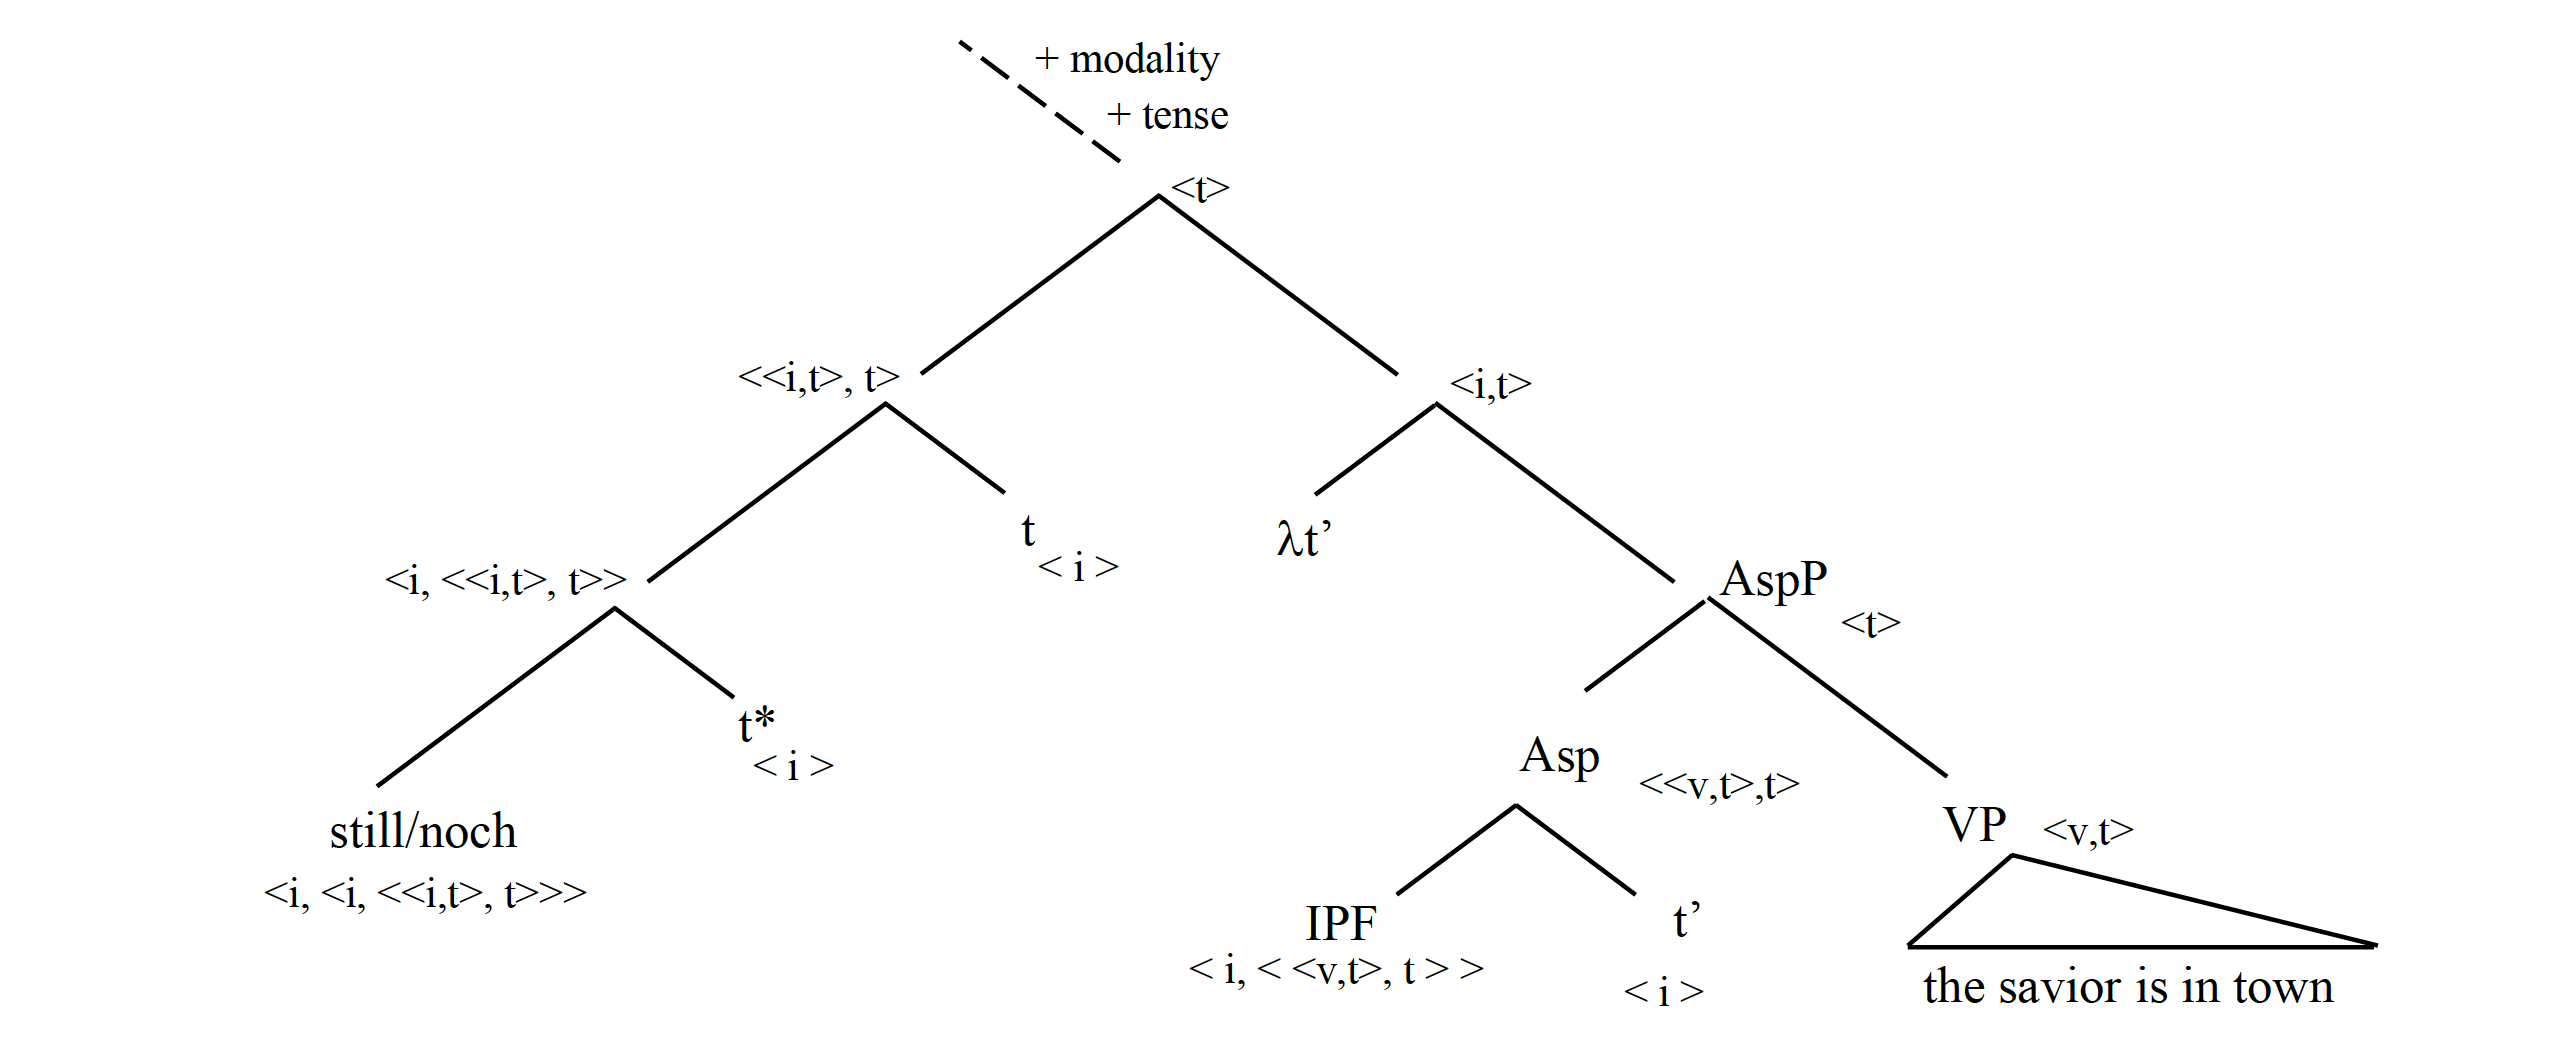
\includegraphics[width=1\textwidth]{figures/LF0_temp}
\caption{LF for \REF{TEMP_jesus_noch_in_town}; cf. \citep{beck2016a_sub}}
\label{fig:LF_TEMP_jesus_noch_in_town}
\end{figure}

\subsection{Stage 2} Let's turn back to example \REF{OG2_noch_mehr_ruehren} (=\ref{OG2_noch_mehr_ruehren_first}) for the following discussion:

\ea\gll Thar uuarun mit githuinge thie iungoron noh tho inne, sie scolta ruaren NOH tho mer thaz selba uuoroltlicha ser.\\
       There were with violence the apostles still there inside, they should move still/even there more the same earthly suffering.\\
\glt   {`The apostles were still inside with violence, they should continue to move/stir the earthly suffering.'}\label{OG2_noch_mehr_ruehren} \hfill (1.OG2.OtfEbKell.351.12)
\z
The \textit{noh} in sentence \REF{OG2_noch_mehr_ruehren} is ambiguous to a temporal and a comparative interpretation. When excluding the comparative operator \textit{mer} (`more') from the interpretation, the temporal continuative interpretation arises with the predicate (`they move/stir the earthly suffering') being true at reference time and a presupposed earlier time (which can be inferred from the context and is overtly satisfied in previous chapters of the stories -- albeit not necessarily in the words of the allegory). In this regard, this is a perfect example since the entire allegory is about the contrast between the earlier time (when Jesus was with the apostles) and the later (reference) time (when Jesus has left the apostles).

The comparative operator in example \REF{OG2_noch_mehr_ruehren} has the effect of comparing the maximum of a property of degrees (subject of comparison/comparee term) to another maximum of a property of degrees (object/comparison base) -- both of type $\langle$d,t$\rangle$ -- with the standard term of comparison being temporally located before reference time.\footnote{ I assume gradable predicates here via a degree argument slot in an adverbial phrase, cf. \figref{fig:LF1_temp_>_over_noch}. I will not go into details as to whether or not (certain) verbs have a degree argument slot or where the degree argument is originating from; for discussion see \citet{pinon2008}, \citet{rett2013}, \citet{KennedyMcNally:2005}, \citet{kennedy2012} and references therein.} The two different points in time are provided by the context since the \textit{than}-clause is covert.

The temporal reading of \textit{noh} puts a condition on the context that at an earlier, presupposed time t* `the apostles move the earthly suffering' and it asserts that `the apostles move the earthly suffering' at reference time t, cf. LF in \figref{fig:LF1_temp_>_over_noch} \citep[cf. also][]{beck2016a_sub}. With the comparative operator having scope over the entire structure, the assertion has to be something like `the apostles move the earthly suffering more than at an earlier time'. Thus, there is a conflict: on the one hand, the temporal \textit{noch} requires a predicate to be true at an earlier time and at reference time and, on the other hand, the comparative requires that the predicate for reference time and an earlier time differs with regard to degrees.

This type of context represents a critical context, i.e. there is an ambiguity and at the same time one reading fits the context better than the other. In \citeauthor{Eckardt_2011}'s \citeyearpar{Eckardt_2011} words, this constitutes a bridging context. In her discussion of reanalysis, she mentions ``precarious uses'' and notes that the criteria for what constitutes a precarious use are manifold -- among other things, they ``can challenge the hearer by pragmatic infelicities'' \citep[44]{Eckardt_2011}.

\begin{figure}
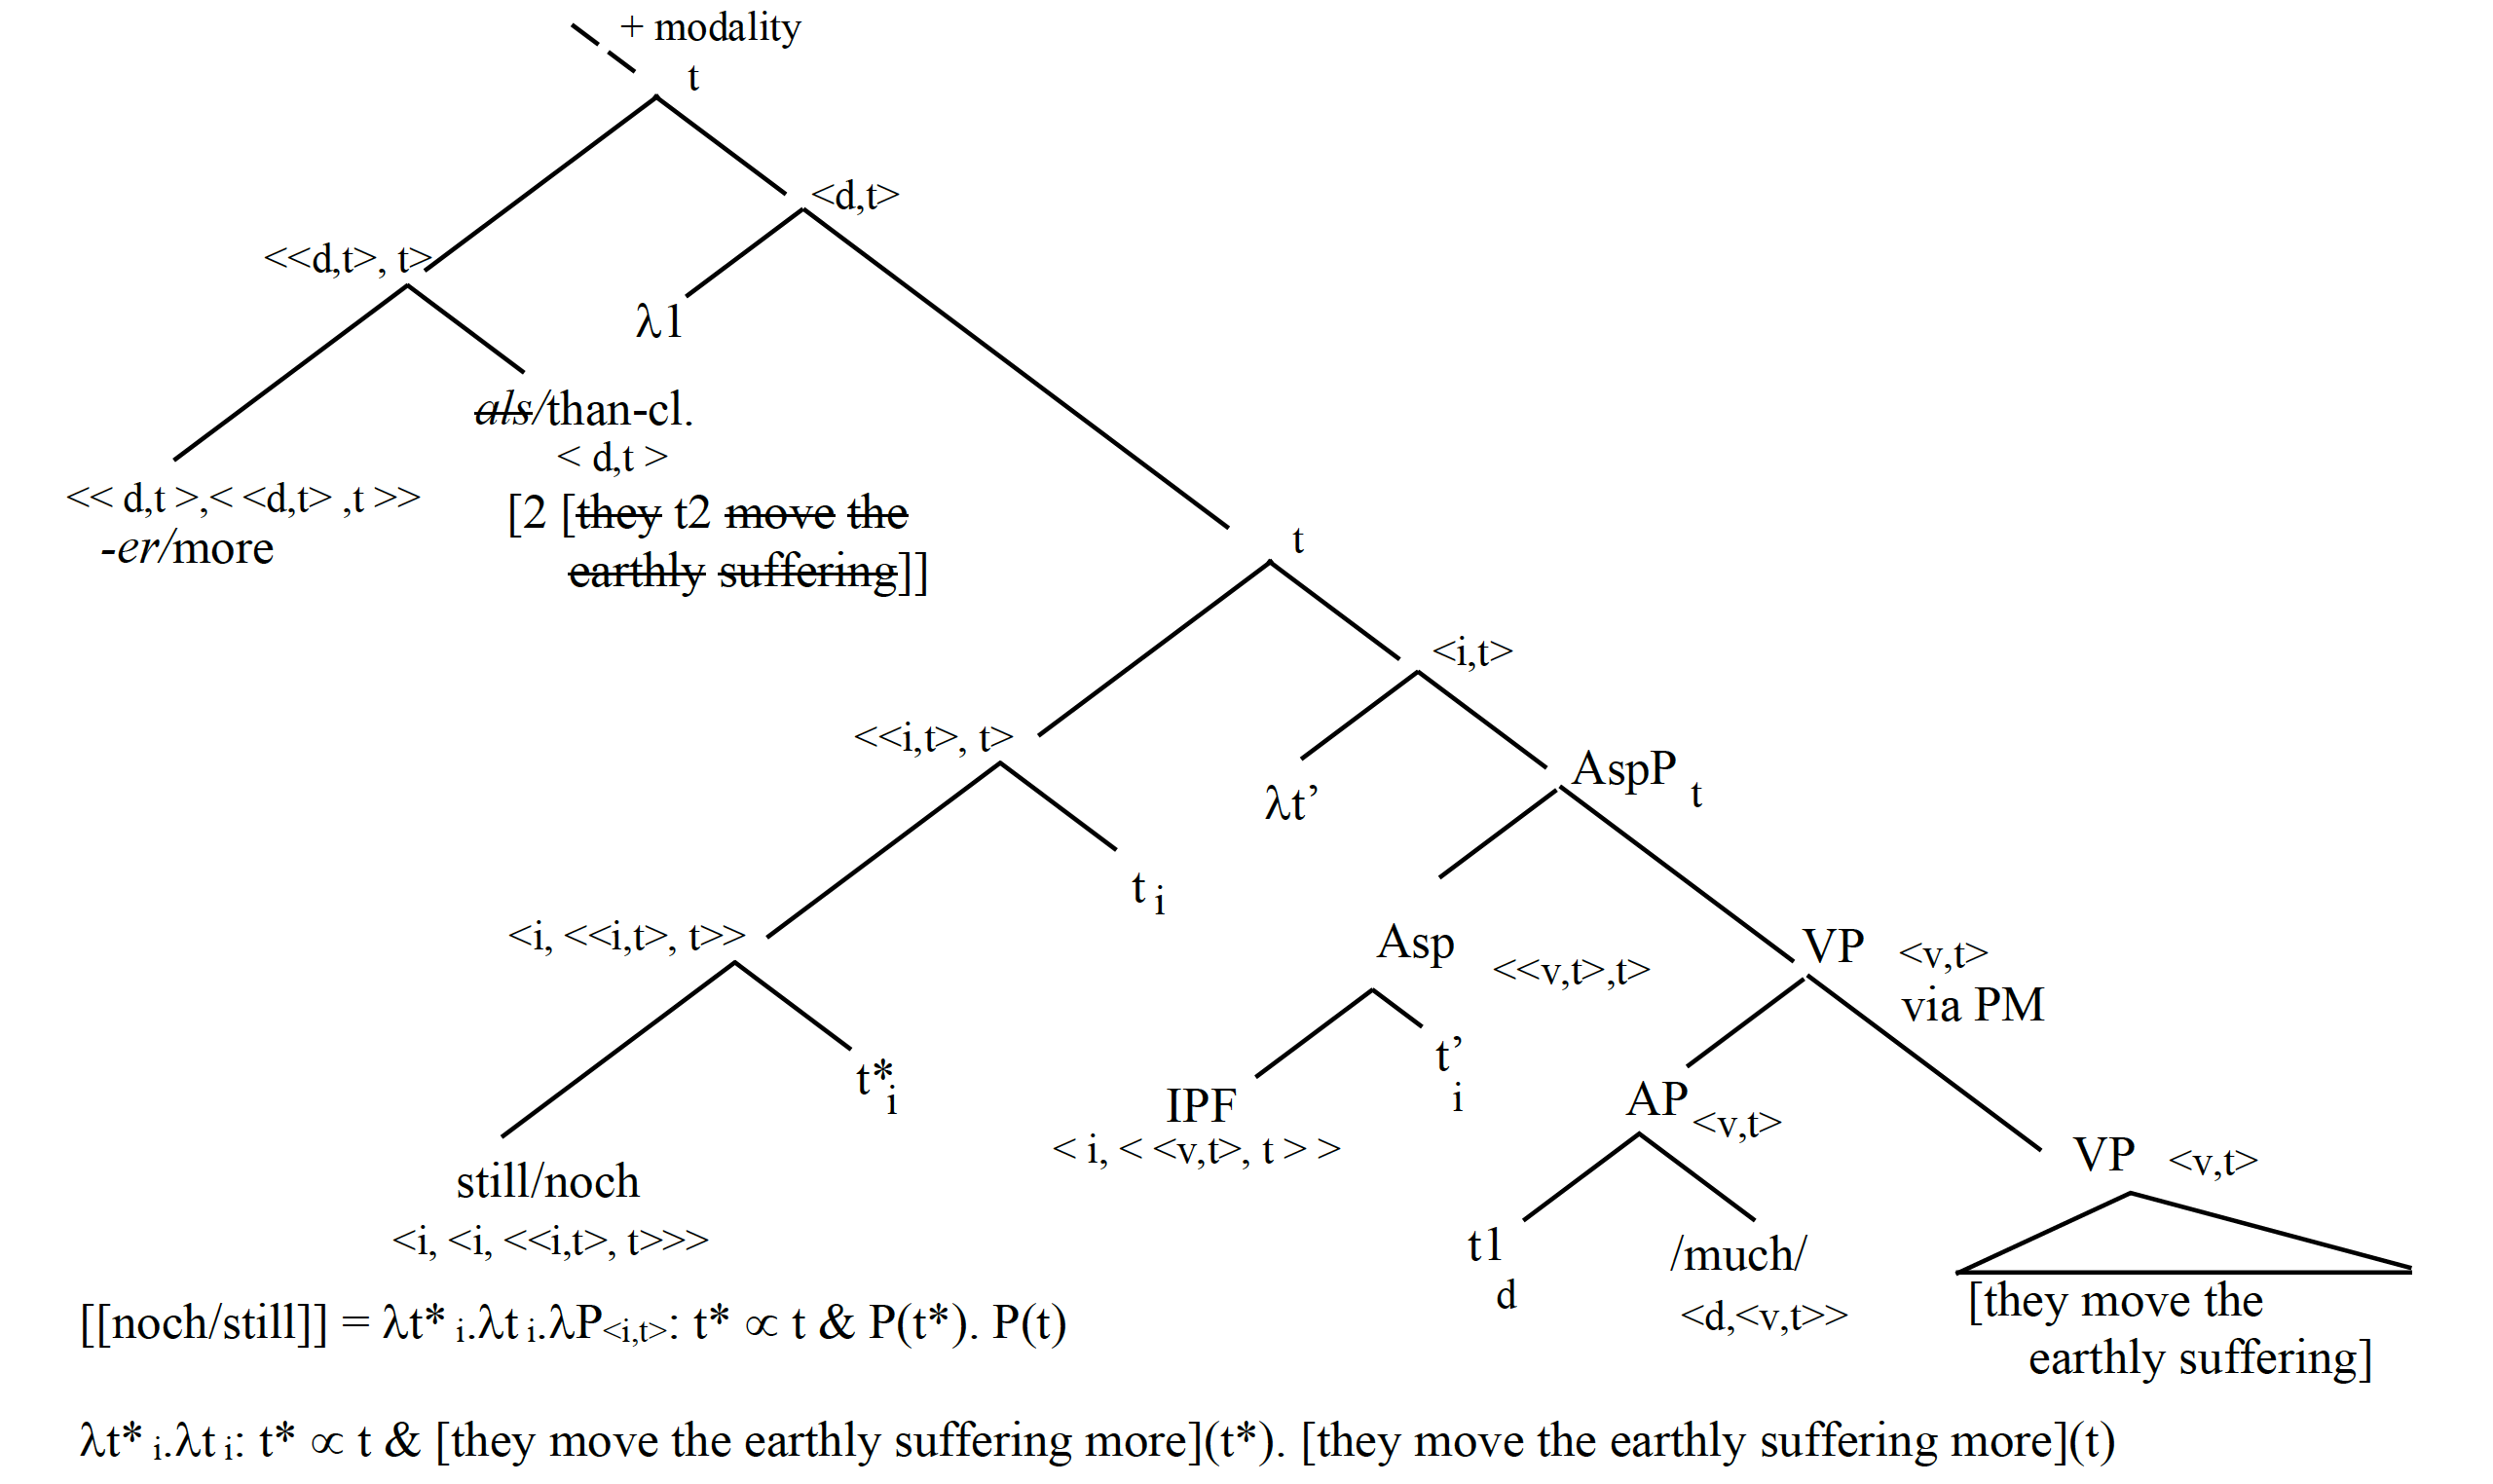
\includegraphics[width=1\textwidth]{figures/LF1_temp_>_over_noch}
\caption{LF for \textit{noch\textsubscript{temp}} for \REF{OG2_noch_mehr_ruehren}; cf. \citep{beck2016a_sub}}
\label{fig:LF1_temp_>_over_noch}
\end{figure}

\subsection{Stage 3} The time interval at reference time becomes reanalyzed as the interval of degrees to which the comparee term and the comparison base differ. As a consequence, the presupposed left-abutting time t* (for which $\text{P}(\text{t*})=1$) becomes reanalyzed as an interval of degrees (on the scale introduced in the matrix clause comparison) to which the comparison base and another, presupposed degree d* differ. The degree d* serves as the lower bound of this second interval of degrees. While \textit{noch}\textsubscript{temp}'s t* is placed at a temporal location lower and relative to reference time (t*<t), \textit{noch}\textsubscript{comp}'s presupposed d* is located lower on a scale of degrees relative to the standard term of comparison ($\text{d*}<\text{max}(\text{D}_{\langle \text{d},\text{t}\rangle}$)). In other words, the interval t* presupposed by \textit{noch}\textsubscript{temp} corresponds to the interval of degrees presupposed by \textit{noch}\textsubscript{comp}, cf. below, \REF{diagram_temp_comp}, and \figref{fig:LF2_comp} for the post-reanalysis LF. The time variable for reference time is interpreted together with the matrix clause, i.e. in the LF below the comparison, as tense. This is necessary since the \textit{than}-clause will have a different tense due to a different temporal location.\footnote{Data like \REF{tense_and_aspect_example} suggests that aspect and tense need to be interpretable below comparison with both clauses having different tenses and aspect. See also \citep{stechow2006}.

\ea \itshape This time \textbf{our guests are staying} longer than \textbf{they stayed} last time. \label{tense_and_aspect_example}\z} Thus, P(t) from the temporal interpretation corresponds to the property of degrees (at present tense) in \REF{OG2_noch_mehr_ruehren} in the comparative interpretation.
It may be argued that the task of pointing to an earlier time is taken over by the comparison which might facilitate for t* to be reanalyzed as the lower bound of another comparison, i.e. another difference in degrees.

\ea\label{diagram_temp_comp}
\ea (Adapted from \citealt{beck2016a_sub})\\\noindent\parbox[t]{\linewidth}{\hspace{43pt} t* \hspace{80pt} t\textsubscript{ref}\\
{-}{-}{-}{-}{-}{-}{-}{-}{-}{-}{-}{-}{-}{-}{-}{-}{-}{-}{-}{-}{-}{-}{-}{-}{-}{-}{-}{-}{-}{|}{-}{-}{-}{-}{-}{-}{-}{-}{-}{-}{-}{-}{-}{-}{-}{-}{-}{-}{-}{-}{-}{-}{|}{-}{-}{-}{-}{-}{-}>\\
P: \hspace{40pt}///////////////////////////////////////\\}
\ex \noindent\parbox[t]{\linewidth}{\hspace{43pt} d* \hspace{30pt} max(D1) \hspace{42pt} max(D2)\\
{-}{-}{-}{-}{-}{-}{-}{-}{-}{-}{-}{-}{-}{º}{-}{-}{-}{-}{-}{-}{-}{-}{-}{-}{-}{-}{-}{-}{-}{º}{-}{-}{-}{-}{-}{-}{-}{-}{-}{-}{-}{-}{-}{-}{-}{-}{-}{-}{-}{-}{-}{-}{º}{-}{-}{-}{-}{-}{-}>\\
ass.: \hspace{85pt}|\hspace{1.125pt}max(D1)<max(D2)\hspace{1.125pt}|\\
PSP: \hspace{25pt}|\hspace{1pt}d*<max(D2)\hspace{1pt}|}
\z\z


A question that has remained unaddressed is, what happens to the rather strong condition that the presupposed time left-abuts reference time (t* $\propto$ t). I argue that it remains intact in the sense that two areas of a scale of degrees are still ordered and adjacent, with the degree of the standard term of comparison being the marker at the boundary between the two different intervals.

Another argument that may be raised is that data like \REF{OG2_noch_mehr_ruehren} say more about future times (times following reference time), rather than reference time or a preceding time t* and, therefore, an analysis of diachronic change should take e.g. \citeauthor{beck2016a_sub}'s \citeyearpar{beck2016a_sub} further-to analysis of \textit{noch}\textsubscript{temp} as a starting point. Here I argue that only due to the fact that the comparative is present some speakers may get this ``forward-directedness''. If \REF{OG2_noch_mehr_ruehren} did not feature a comparative operator, the continuative reading of \textit{noch}\textsubscript{temp} would give the right predictions and be perfectly satisfied by the context.


\begin{figure}
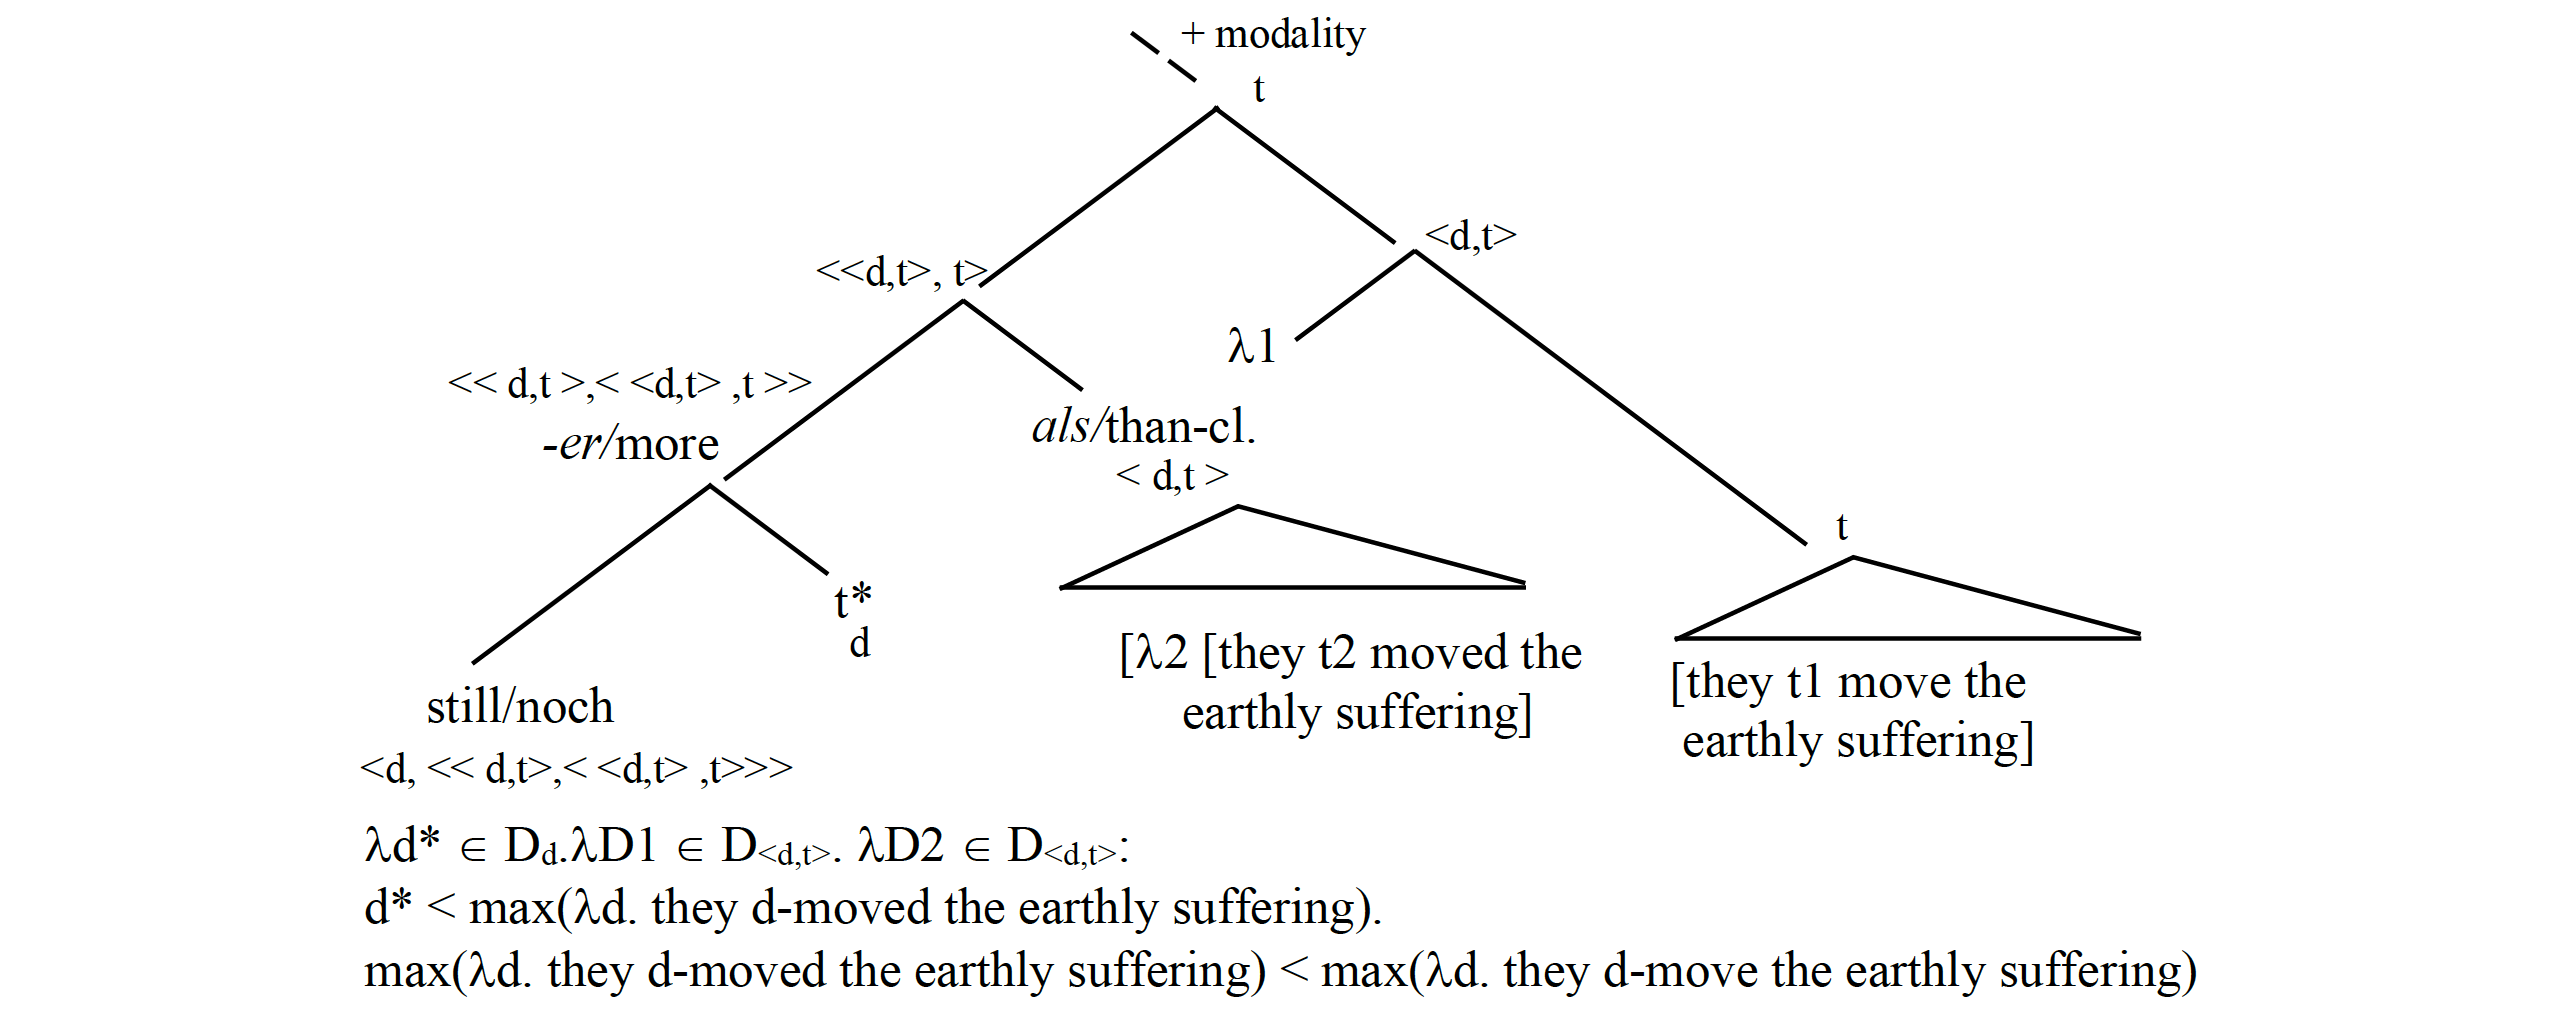
\includegraphics[width=1\textwidth]{figures/LF2_comp}
\caption{LF for \textit{noch\textsubscript{comp}} for \REF{OG2_noch_mehr_ruehren}; cf. \citep{beck2016a_sub}}
\label{fig:LF2_comp}
\end{figure}

\subsection{Stage 4} Unambiguous \textit{noch}\textsubscript{comp} is available as early as OG3 (950--1050). The context for \REF{OG3_noch_more_glory} is that God took Jesus to him when he died among the humans. After that the christian church/religion is endowed with glory (since Jesus has lifted all sins from the humans) and Jesus is also endowed with (even more) glory because he sits next to God for eternity. \REF{OG3_noch_more_glory} does not license a temporal reading. As with the previous example, there is an antecedent comparison where the degree to which the church has glory is compared to a standard degree of glory.

\ea\gll Michel ist íro guôllichi an dînemo haltâre christo. [Lat.] Ímo selbemo gíbest du noh mêrun guôllichi. unde mêrun ziêreda. sô dû in gesezzest ad dexteram tuam.\\
       great is her glory in your savior christ [Lat.] him self give you still/even more glory. and more adornment. as you him set to\_LAT right\_LAT your\_LAT.\\
\glt   {`Great is the glory of the church in your savior christ. You give him still/even more glory and more adornment by setting him at your right side.'}\label{OG3_noch_more_glory} \hfill (1.OG3.N:Ps:20.61-63)
\z

\begin{figure}
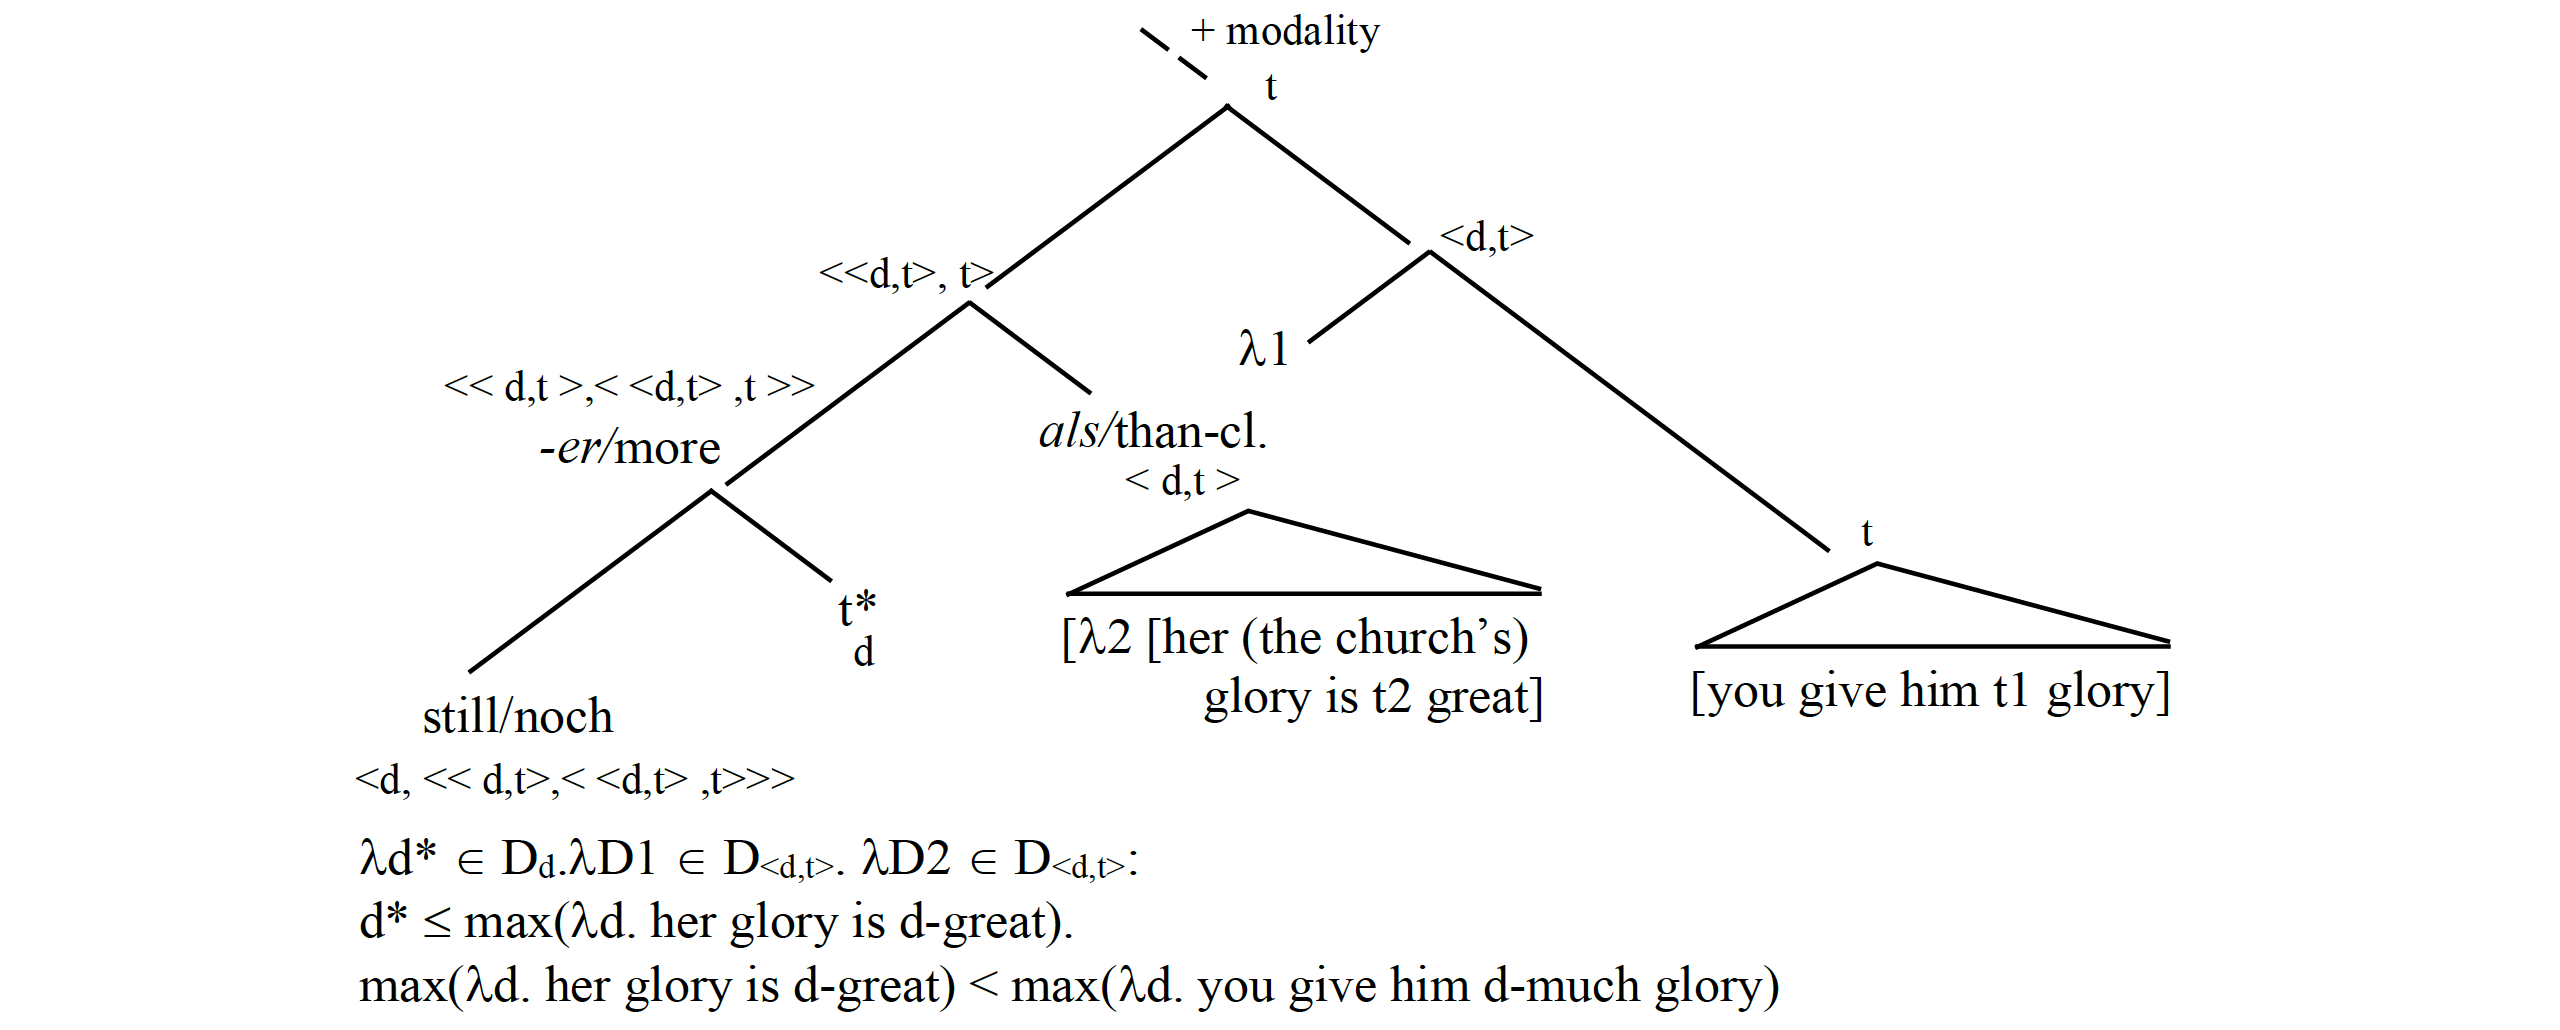
\includegraphics[width=1\textwidth]{figures/LF3_comp}
\caption{LF for \REF{OG3_noch_more_glory}; cf. \citep{beck2016a_sub}}
\label{fig:LF3_comp}
\end{figure}

In the OG3 subperiod, the modern German interpretation of \textit{noch}\textsubscript{comp} is fully available. The \textit{no(c)h} in \REF{OG3_noch_more_glory} together with its context does not allow a temporal reading any longer. This is in contrast to the earlier examples from OG2.

\section{Conclusion}

The above aims to contribute to the understanding of the semantics of \textit{noch}\textsubscript{comp}. I reported on an experiment investigating the PSP component of this use of \textit{noch} and attempted to consolidate the findings with existing contributions to its semantics. Moreover, the experiment has informed the diachronic discussion of \textit{noch}\textsubscript{comp} in the sense that it provided direction for \textit{noch}'s diachronic trajectory. For this trajectory, I have proposed a process of reanalysis for the comparative reading of \textit{noch} as having developed from the temporal reading of \textit{noch}. The above proposal is motivated by the ambiguity between temporal and comparative readings of the earliest examples comparative readings of \textit{no(c)h} available. Despite the empirical evidence being rather limited, there are a number of aspects that support the above proposal. Many things need further investigation, among others: the additive use of \textit{noch} and its diachrony need detailed corpus based research in order to (i) better understand when and how it arose and (ii) its possible entanglement with the development of the comparative use of \textit{noch}. \citeauthor{beck2016a_sub}'s \citeyearpar{beck2016a_sub} discussion of a variety of temporal readings leading up to additivity of \textit{noch} provides a plausible diachronic trajectory for the development \textit{noch}\textsubscript{add} which, in turn, (iii) requires a more thorough look at the data on \textit{noch}\textsubscript{temp}. Furthermore, \textit{noch}\textsubscript{comp} needs investigating in later periods as well.


{\sloppy\printbibliography[heading=subbibliography,notkeyword=this]}



\section*{Appendix}
\tabref{tab:16_contexts} contains all the condition-3-target items for all 16 token sets. For space constraints I can only include one condition. However, based on Tables~\ref{tab:16_contexts} and~\ref{tab:4_conds} (p. \pageref{tab:4_conds}) it is straightforward to reconstruct the remaining conditions as \tabref{tab:emil_example} exemplifies by means of the first toke set in line no. 01 in \tabref{tab:16_contexts}.



\begin{longtable}{lp{317.90625pt}}
\caption{Experimental design; condition-3-target items (fac 1, lev 2 \& fac 2, lev 2) for 16 token sets\label{tab:16_contexts}}\\
\lsptoprule no. & target item \& and translation\\\midrule\endfirsthead\midrule no. & target item \& and translation\\\midrule\endhead\endfoot\lspbottomrule\endlastfoot
01 & Emil ist größer als Felix und Georg ist noch größer als Emil. Dabei ist Emil nicht groß. \\
   & {`Emil is taller than Felix and George is still taller than Emil. And yet Emil is not tall.'}\\
\midrule
02 & Sarah ist kleiner als Tina und Ulrike ist noch kleiner als Sarah. Dabei ist Sarah nicht klein.\\
   & {`Sarah is shorter than Tina and Ulrike is still shorter than Sarah. And yet Sarah is not short.'}\\
\midrule
03 & Die Birke ist höher als die Eiche und die Fichte ist noch höher als die Birke. \\
   & Dabei ist die Birke nicht hoch.\\
   & {`The birch tree is taller than than the oak tree and the spruce is still taller than the birch tree.}\\
   & \textit{And yet the birch is not tall.'}\\
\midrule
04 & Die Goldmine ist tiefer als die Kupfermine und die Salzmine ist noch tiefer als die Goldmine. \\
   & Dabei ist die Goldmine nicht tief. \\
   & {`The gold mine is deeper than the copper mine and the salt mine is still deeper than the gold mine.} \\
   & {And yet the gold mine is not deep.'}\\
\midrule
05 & Das Sofa ist breiter als der Tisch und das Regal ist noch breiter als das Sofa. Dabei ist das Sofa nicht breit.\\
   & {`The sofa is wider than the table and the shelf is still wider than the sofa. And yet the sofa is not wide.'}\\
\midrule
06 & Das Fenster ist schmaler als der Gang und die Türe ist noch schmaler als das Fenster.\\
   & Dabei ist das Fenster nicht schmal.\\
   & {`The window is narrower than the hallway and the door is still narrower than the winder.} \\
   & {And yet the window is not narrow.'}\\
\midrule
07 & Der Rhein ist länger als die Elbe und die Donau ist noch länger als der Rhein. Dabei ist der Rhein nicht lang.\\
   & {`The Rhine is longer than the Elbe and the Danube is still longer than the Rhine. And yet the Rhine is not long.'}\\
\midrule
08 & Das Kabel ist kürzer als der Draht und das Seil ist noch kürzer als das Kabel. Dabei ist das Kabel nicht kurz.\\
   & {`The cord is shorter than the wire and the rope is still shorter than the cord. And yet the cord is not short.'}\\
\midrule
09 & Doris ist schneller als Elsa und Flora ist noch schneller als Doris. Dabei ist Doris nicht schnell.\\
   & {`Doris is faster than Elsa and Flora is still faster than Doris. And yet Doris is not fast.'}\\
\midrule
10 & Oskar ist langsamer als Peter und Robert ist noch langsamer als Oskar. Dabei ist Oskar nicht langsam.\\
   & {`Oscar is slower than Peter and Robert is still slower than Oscar. And yet Oscar is not slow.'}\\
\midrule
11 & Konrad ist jünger als Lukas und Max ist noch jünger als Konrad. Dabei ist Konrad nicht jung.\\
   & {`Conrad is younger than Lucas and Max is still younger than Conrad. And yet Conrad is not young.'}\\
\midrule
12 & Gina ist älter als Hannah und Ilse ist noch älter als Gina. Dabei ist Gina nicht alt.\\
   & {`Gina is older than Hannah and Ilse is still older than Gina. And yet Gina is not old.'} \\
\midrule
13 & Das Buch ist besser als das Musical und der Film ist noch besser als das Buch. Dabei ist das Buch nicht gut.\\
   & {`The book is better than the musical and the movie is still better than the book. And yet the book is not good.'} \\
\midrule
14 & Das Buch ist schlechter als das Musical und der Film ist noch schlechter als das Buch. Dabei ist das Buch nicht schlecht.\\
   & {`The book is worse than the musical and the movie is still worse than the book. And yet the book is not bad.'} \\
\midrule
15 & Die 'Mona Lisa' ist schöner als 'Die Geburt der Venus' und 'Sternennacht' ist noch schöner als die 'Mona Lisa'. \\
   & Dabei ist die 'Mona Lisa' nicht schön. \\
   & {`The Mona Lisa is more beautiful than The Birth of Venus and The Starry Night is still more beautiful than The Mona Lisa.'}\\
   & {`And yet The Mona Lisa is not beautiful.'}\\
\midrule
16 & Das T-Shirt ist hässlicher als die Jeans und der Pullover ist noch hässlicher als das T-Shirt. Dabei ist das T-Shirt nicht hässlich.\\
   & {`The t-shirt is uglier than the jeans and the pullover is still uglier than the t-shirt. And yet the t-shirt is not ugly.'}\\
\end{longtable}


\begin{sidewaystable}
\begin{tabular}{lllll}
\lsptoprule
cond & fac 1 & fac 2 & item & \\
\midrule
1 & \texttt{ass} & \texttt{+n} & Emil ist groß \hspace{25pt} und Georg ist noch größer als Emil. & Dabei ist Emil nicht groß. \\
 & & & {`Emil is tall \hspace{32pt} and George is \hspace{0.4pt} still \hspace{2pt} taller than Emil.} & \textit{And yet Emil is not tall.'} \\
\midrule
2 & \texttt{ass} & \texttt{-n} & Emil ist groß \hspace{25pt} und Georg ist \hspace{16pt} größer als Emil. & Dabei ist Emil nicht groß. \\
 & & & {`Emil is tall \hspace{32pt} and George is \hspace{19pt} taller than Emil.} & \textit{And yet Emil is not tall.'}   \\
\midrule
3 & \texttt{com} & \texttt{+n} & Emil ist größer als Felix \hspace{0.65pt} und Georg ist noch größer als Emil. & Dabei ist Emil nicht groß.   \\
 & & & {`Emil is taller than Felix \hspace{2pt} and George is \hspace{0.4pt} still \hspace{2pt} taller than Emil.} & \textit{And yet Emil is not tall.'}  \\
\midrule
4 & \texttt{com} & \texttt{-n} & Emil ist größer als Felix \hspace{0.65pt} und Georg ist \hspace{16pt} größer als Emil. & Dabei ist Emil nicht groß.   \\
 & & & {`Emil is taller than Felix \hspace{2pt} and George is \hspace{19pt} taller than Emil.} & \textit{And yet Emil is not tall.'}   \\
\lspbottomrule
\end{tabular}
\caption{example, 4 conditions  per token set (fac 1, lev 2 \& fac 2, lev 2)}
\label{tab:emil_example}
\end{sidewaystable}


\noindent The following shows the combinatorics behind the compilation of the questionnaires (A -- H). The goal was to minimize response fatigue and reduce questionnaire duration. Therefore, I ended up with 8 questionnaires, each containing 8 target items and 16 fillers. The 64 target items were rotated/pseudo-randomized among the questionnaire groups, cf. \tabref{tab:questionnaire_combos}, below. This was done to ensure that every participant had to rate 8 items with the conditions: (i) never seeing any token set more than once, (ii) rating every condition twice, (iii) at least one item from every antonymous token set pair (i.e.: token set 1 -- \textit{tall} \& token set 2 -- \textit{short}).

\begin{table}
\begin{tabular}{cccccccc}
\lsptoprule
item no. & token set & cond. & \textbf{quest.} & item no. & token set & cond. & \textbf{quest.} \\
\midrule \midrule
1  & 1 & 1 & \textit{A}     & 33 & 9 & 1 & \textit{E}\\
2  & 1 & 2 & \textit{B}     & 34 & 9 & 2 & \textit{F} \\
3  & 1 & 3 & \textit{C}     & 35 & 9 & 3 & \textit{G} \\
4  & 1 & 4 & \textit{D}     & 36 & 9 & 4 & \textit{H} \\
5  & 2 & 1 & \textit{E}     & 37 & 10 & 1 & \textbf{A} \\
6  & 2 & 2 & \textit{F}     & 38 & 10 & 2 & \textbf{B} \\
7  & 2 & 3 & \textit{G}     & 39 & 10 & 3 & \textbf{C} \\
8  & 2 & 4 & \textit{H}     & 40 & 10 & 4 & \textbf{D} \\ \midrule
9  & 3 & 1 & \textit{B}     & 41 & 11 & 1 & \textit{F} \\
10  & 3 & 2 & \textit{C}    & 42 & 11 & 2 & \textit{G} \\
11  & 3 & 3 & \textit{D}    & 43 & 11 & 3 & \textit{H} \\
12  & 3 & 4 & \textit{E}    & 44 & 11 & 4 & \textbf{A} \\
13  & 4 & 1 & \textit{F}    & 45 & 12 & 1 & \textbf{B} \\
14  & 4 & 2 & \textit{G}    & 46 & 12 & 2 & \textbf{C} \\
15  & 4 & 3 & \textit{H}    & 47 & 12 & 3 & \textbf{D} \\
16  & 4 & 4 & \textbf{A}    & 48 & 12 & 4 & \textbf{E} \\ \midrule
17  & 5 & 1 & \textit{C}    & 49 & 13 & 1 & \textit{G} \\
18  & 5 & 2 & \textit{D}    & 50 & 13 & 2 & \textit{H} \\
19  & 5 & 3 & \textit{E}    & 51 & 13 & 3 & \textbf{A} \\
20  & 5 & 4 & \textit{F}    & 52 & 13 & 4 & \textbf{B} \\
21 & 6 & 1 & \textit{G}     & 53 & 14 & 1 & \textbf{C} \\
22 & 6 & 2 & \textit{H}     & 54 & 14 & 2 & \textbf{D} \\
23 & 6 & 3 & \textbf{A}     & 55 & 14 & 3 & \textbf{E} \\
24 & 6 & 4 & \textbf{B}     & 56 & 14 & 4 & \textbf{F} \\ \midrule
25 & 7 & 1 & \textit{D}     & 57 & 15 & 1 & \textit{H} \\
26 & 7 & 2 & \textit{E}     & 58 & 15 & 2 & \textbf{A} \\
27 & 7 & 3 & \textit{F}     & 59 & 15 & 3 & \textbf{B} \\
28 & 7 & 4 & \textit{G}     & 60 & 15 & 4 & \textbf{C} \\
29 & 8 & 1 & \textit{H}     & 61 & 16 & 1 & \textbf{D} \\
30 & 8 & 2 & \textbf{A}     & 62 & 16 & 2 & \textbf{E} \\
31 & 8 & 3 & \textbf{B}     & 63 & 16 & 3 & \textbf{F} \\
32 & 8 & 4 & \textbf{C}     & 64 & 16 & 4 & \textbf{G} \\
\lspbottomrule
\end{tabular}
\caption{Combination of token sets and conditions into questionnaires. quest. = questionnaire}
\label{tab:questionnaire_combos}
\end{table}


\end{document}
